\documentclass[11pt]{report}
% Shared preamble for the Superstore ML report.
\usepackage[a4paper,margin=2.5cm]{geometry}
\usepackage[utf8]{inputenc}
\usepackage[T1]{fontenc}
\usepackage{lmodern}
\usepackage{amsmath,amssymb,amsthm}
\usepackage{graphicx}
\usepackage{booktabs}
\usepackage{array}
\usepackage{caption}
\usepackage{subcaption}
\usepackage{xcolor}
\usepackage[colorlinks=true,linkcolor=blue!50!black,citecolor=blue!50!black,urlcolor=blue!50!black]{hyperref}
\usepackage{fancyhdr}
\usepackage{titlesec}
\usepackage{enumitem}
\usepackage{listings}
\usepackage{algorithm}
\usepackage{algpseudocode}
\usepackage{float}
\usepackage{siunitx}
\usepackage[capitalise]{cleveref}

\graphicspath{{../outputs/figures/}}

\setlength{\parskip}{0.4em}
\setlength{\parindent}{1.2em}

\pagestyle{fancy}
\fancyhf{}
\fancyhead[L]{\small\nouppercase{\leftmark}}
\fancyhead[R]{\small Superstore End-to-End ML Report}
\fancyfoot[C]{\thepage}
\renewcommand{\headrulewidth}{0.4pt}

\newtheorem{definition}{Definition}[section]
\newtheorem{theorem}{Theorem}[section]
\newtheorem{remark}{Remark}[section]

\lstset{
  basicstyle=\ttfamily\footnotesize,
  breaklines=true,
  frame=single,
  columns=fullflexible,
  backgroundcolor=\color{gray!8},
}

\captionsetup{font=small,labelfont=bf}


\title{\textbf{End-to-End Machine Learning on Retail Transaction Data}\\[0.3em]
       \large A Theory-and-Results Report on the Sample Superstore Dataset}
\author{Debarshi Chakraborty}
\date{\today}

\begin{document}

\begin{titlepage}
  \centering
  \vspace*{2cm}
  {\Huge\bfseries End-to-End Machine Learning on Retail Transaction Data\par}
  \vspace{0.6cm}
  {\Large A Theory-and-Results Report on the Sample Superstore Dataset\par}
  \vspace{2cm}
  {\large Debarshi Chakraborty\par}
  \vspace{0.3cm}
  {\large \today\par}
  \vfill
  {\large
    Companion codebase: \texttt{EY Training/ml\_superstore/}\\
    Data: \texttt{EY Training/data/Sample - Superstore.csv} (9{,}994 order lines, 2014--2017, USA)
  \par}
  \vspace{1cm}
\end{titlepage}

\pagenumbering{roman}
\begin{abstract}
\noindent
This report documents an end-to-end machine learning study built on the
Sample Superstore retail dataset. It follows the same five stages as the
accompanying Jupyter notebooks and source package
(\texttt{EY Training/ml\_superstore/}): data ingestion and quality
assessment, exploratory data analysis, feature engineering, time-series
forecasting of monthly sales, and supervised learning for line-level profit
prediction and loss detection. Unlike the notebooks, whose purpose is
interactive exploration, this report is written to stand alone: every
technique used is first introduced from first principles --- the statistical
or algorithmic theory it rests on --- and only then applied to the data,
with the resulting figures, tables and their business interpretation
presented immediately afterwards. The headline findings are that (i) order
discounting beyond roughly 30\% is the dominant driver of loss-making order
lines, far outweighing category, region or shipping mode; (ii) an additive
Holt--Winters exponential smoothing model forecasts monthly sales with an
out-of-sample MAPE of approximately 23\%, competitive with a seasonal
ARIMA model and clearly better than a seasonal-naive baseline; and (iii) a
random-forest classifier trained on leakage-safe features identifies
loss-making order lines with a PR-AUC of 0.96 on a strictly future
(2017) hold-out year, giving a concrete, auditable basis for a discount
governance policy.
\end{abstract}

\tableofcontents
\listoffigures
\listoftables

\clearpage
\pagenumbering{arabic}

\chapter{Introduction}
\label{ch:intro}

\section{Objective}
Retail order-line data — one row per product sold within an order — sits at
the intersection of three classical machine-learning problem types:
descriptive analytics (what happened), predictive analytics (what will
happen), and diagnostic/prescriptive analytics (why it happened, and what
to do about it). This report uses the public \emph{Sample Superstore}
dataset to walk through all three, mirroring a realistic analytics
engagement:

\begin{enumerate}[label=\arabic*.]
  \item \textbf{Data quality and exploratory analysis} — establish that the
        data is trustworthy and characterise its statistical structure.
  \item \textbf{Feature engineering} — turn raw transactional fields into
        model-ready predictors, with explicit attention to information
        leakage.
  \item \textbf{Forecasting} — model and project the aggregate monthly
        sales time series.
  \item \textbf{Supervised learning} — model two line-level targets,
        \emph{profit} (regression) and \emph{is a line loss-making}
        (classification), and interpret what drives them.
\end{enumerate}

Each stage in this report is structured identically: a \textbf{Theory}
section derives or states the relevant statistical/ML machinery from first
principles, followed by a \textbf{Method} section describing how it was
applied to this dataset, then \textbf{Results} with the produced figures
and tables, and finally an \textbf{Interpretation} section connecting the
numbers back to a business reading. This mirrors, chapter for chapter, the
five numbered notebooks in \texttt{EY\_Training/ml\_superstore/notebooks/}
and the reusable modules in \texttt{src/}.

\section{Dataset}
The dataset contains $n = 9{,}994$ order lines spanning
\SI{4}{years} (2014--01--03 to 2017--12--30), $793$ unique customers and
$1{,}862$ unique products, organised into $5{,}009$ distinct orders across
the United States. Table~\ref{tab:intro-schema} summarises the raw schema.

\begin{table}[H]
  \centering
  \caption{Raw schema of the Sample Superstore CSV.}
  \label{tab:intro-schema}
  \begin{tabular}{@{}llp{7.5cm}@{}}
    \toprule
    \textbf{Field} & \textbf{Type} & \textbf{Description} \\
    \midrule
    Row ID, Order ID & id & Line and order identifiers \\
    Order Date, Ship Date & date & Order placement and shipment dates \\
    Ship Mode & categorical & Standard / Second / First Class, Same Day \\
    Customer ID, Customer Name & id/text & Buyer identity \\
    Segment & categorical & Consumer / Corporate / Home Office \\
    Country, City, State, Postal Code, Region & geography & U.S. location fields \\
    Product ID, Category, Sub-Category, Product Name & catalogue & 3-level product hierarchy \\
    Sales & numeric (\$) & Line revenue \\
    Quantity & numeric & Units sold \\
    Discount & numeric $[0,1)$ & Fractional discount applied \\
    Profit & numeric (\$) & Line profit (can be negative) \\
    \bottomrule
  \end{tabular}
\end{table}

\section{Software and reproducibility}
All analysis is implemented in Python 3.10 using \texttt{pandas},
\texttt{numpy}, \texttt{scikit-learn}, \texttt{statsmodels},
\texttt{matplotlib}/\texttt{seaborn}. Code lives in
\texttt{EY\_Training/ml\_superstore/src/} as importable modules
(\texttt{data\_loader}, \texttt{features}, \texttt{forecasting},
\texttt{modeling}, \texttt{pipeline}), exercised interactively by six
Jupyter notebooks and, for one-shot reproduction, by
\texttt{python -m src.pipeline}. Every figure reproduced in this report was
generated by that codebase and saved under \texttt{outputs/figures/}; every
number quoted in the text is read directly from the corresponding CSV in
\texttt{outputs/tables/} or the machine-written \texttt{outputs/REPORT.md}.
No figure or statistic in this document was computed by hand.

\section{Notation}
Throughout, $y_i$ denotes a target value for observation $i$,
$\hat y_i$ its model prediction, $\mathbf{x}_i \in \mathbb{R}^p$ its feature
vector, and $n$ the sample size of the set under discussion (which may be a
train, test, or full-data set, made explicit in context). For the monthly
sales series we write $y_t$, $t = 1, \dots, T$, for the value in month $t$.
$\mathbb{E}[\cdot]$, $\mathrm{Var}(\cdot)$ and $\mathrm{Cov}(\cdot,\cdot)$
denote expectation, variance and covariance under whatever probabilistic
model is being assumed at that point (population model for theory,
empirical/plug-in estimator when applied to data).

\chapter{Data Quality and Exploratory Analysis}
\label{ch:eda}

\section{Theory}

\subsection{Data quality auditing}
Before any modelling, three questions must be answered about a tabular
dataset $D = \{(\mathbf{x}_i)\}_{i=1}^n$: (i) is every field typed and
parsed correctly, (ii) is any value missing, and (iii) is any row
duplicated. Formally, for a column $X$ we report the \emph{missingness
rate} $\hat\pi_X = \frac{1}{n}\sum_{i=1}^n \mathbb{1}[x_{i} \text{ is
NA}]$ and \emph{cardinality} $|\{x_i\}|$. A duplicate row under a primary
key $k$ is any pair $i \neq j$ with $k_i = k_j$; if such pairs exist, the
key does not uniquely identify a record and downstream joins or grouped
aggregates will silently double-count. These checks are cheap and
guard against exactly the class of error (a re-exported CSV with
duplicated header rows, an encoding mismatch producing NA in a text field)
that otherwise corrupts every later stage silently.

\subsection{Descriptive statistics and distribution shape}
For a numeric column $X$ with observed values $x_1,\dots,x_n$, the sample
mean $\bar x = \frac1n\sum_i x_i$ and variance
$s^2 = \frac{1}{n-1}\sum_i (x_i-\bar x)^2$ summarise location and spread,
but retail money variables are rarely well described by them alone because
they are \emph{right-skewed}: many small transactions and a long tail of
large ones. Skewness is measured by the third standardised moment,
\begin{equation}
  \gamma_1 = \frac{\frac1n\sum_i (x_i - \bar x)^3}{\left(\frac1n\sum_i (x_i-\bar x)^2\right)^{3/2}},
  \label{eq:skew}
\end{equation}
with $\gamma_1 > 0$ indicating a right tail. A common remedy that
stabilises both skew and the variance-vs-mean relationship
(heteroscedasticity) seen in multiplicative processes like sales is the
$\log(1+x)$ transform, used throughout this project on \texttt{Sales}
(and, with a sign-preserving variant, on \texttt{Profit}) purely for
\emph{visualisation}; models are always trained on the original scale
unless stated otherwise, since tree ensembles are invariant to monotone
transforms and linear models' coefficients are more directly interpretable
untransformed here.

\subsection{Correlation}
For two numeric variables $X, Y$, the Pearson correlation coefficient
\begin{equation}
  \rho_{XY} = \frac{\mathrm{Cov}(X,Y)}{\sigma_X \sigma_Y}
            = \frac{\sum_i (x_i - \bar x)(y_i - \bar y)}
                   {\sqrt{\sum_i (x_i-\bar x)^2}\sqrt{\sum_i (y_i-\bar y)^2}}
  \label{eq:pearson}
\end{equation}
measures \emph{linear} association, $\rho_{XY}\in[-1,1]$. It is
insensitive to non-linear relationships (e.g. a U-shape can have
$\rho \approx 0$ despite strong dependence), which is precisely why
\cref{sec:eda-discount-profit} supplements the correlation matrix with a
binned conditional-mean plot: discount and profit turn out to have a
threshold-like, not linear, relationship.

\subsection{Seasonal-trend decomposition (STL)}
A time series $y_t$ is classically modelled as the additive sum of a
slowly-varying trend $T_t$, a periodic seasonal component $S_t$ (period
$L$, here $L=12$ months), and a remainder $R_t$:
\begin{equation}
  y_t = T_t + S_t + R_t.
  \label{eq:stl-additive}
\end{equation}
\textbf{STL} (Seasonal-Trend decomposition using \textsc{Loess}, Cleveland
et al., 1990) estimates $T_t$ and $S_t$ by alternating two local
regression (LOESS) smooths: it removes a running estimate of $T_t$ from
$y_t$ to expose the seasonal cycle, smooths within each seasonal
sub-series (all Januaries, all Februaries, \dots) to obtain a smoothly
time-varying $S_t$, then smooths $y_t - S_t$ to update $T_t$; this is
iterated to convergence. Unlike a single global seasonal index, STL lets
the seasonal shape drift slowly over the four years of data, and unlike
classical decomposition it is robust to outliers when the \texttt{robust}
option down-weights large residuals between iterations. We use STL purely
as a diagnostic here; the forecasting models of \cref{ch:forecasting} are
fitted directly on $y_t$, not on the decomposed components.

\section{Method}
The raw CSV is read with \texttt{src.data\_loader.load\_raw} (encoding
auto-detection across UTF-8/Latin-1/CP1252) and typed with \texttt{clean},
which parses \texttt{Order Date}/\texttt{Ship Date}, strips whitespace from
every text column, drops exact and \texttt{Row ID} duplicates, and derives
\texttt{Ship Days} $= \text{Ship Date} - \text{Order Date}$. The quality
audit, univariate/bivariate plots and STL decomposition are produced by
notebooks \texttt{01\_data\_overview.ipynb} and \texttt{02\_eda.ipynb}.

\section{Results}

\subsection{Data quality}
The audit (\texttt{outputs/tables/01\_data\_quality.csv}) finds
\textbf{zero missing values in any of the 21 raw columns}, no fully
duplicated rows, and no duplicate \texttt{Row ID}s after cleaning — the
data is analysis-ready without imputation. \texttt{Order Date} spans
2014-01-03 to 2017-12-30 (1{,}237 distinct dates); \texttt{Ship Days} is
always non-negative, i.e. no order ships before it is placed.

\subsection{Distributions}
\begin{figure}[H]
  \centering
  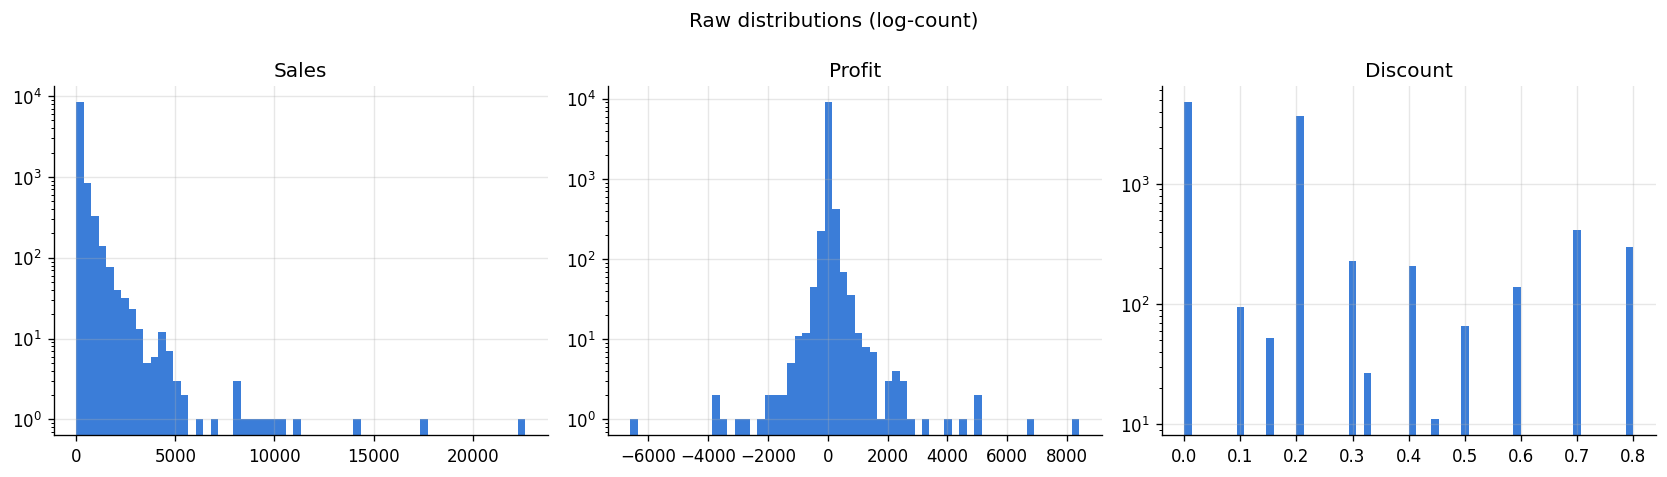
\includegraphics[width=0.95\linewidth]{01_raw_distributions.png}
  \caption{Histograms (log-count $y$-axis) of \texttt{Sales}, \texttt{Profit}
  and \texttt{Discount} on the raw scale, showing pronounced right skew in
  \texttt{Sales} and a bimodal, discount-tier structure in \texttt{Discount}.}
  \label{fig:raw-dist}
\end{figure}

\begin{figure}[H]
  \centering
  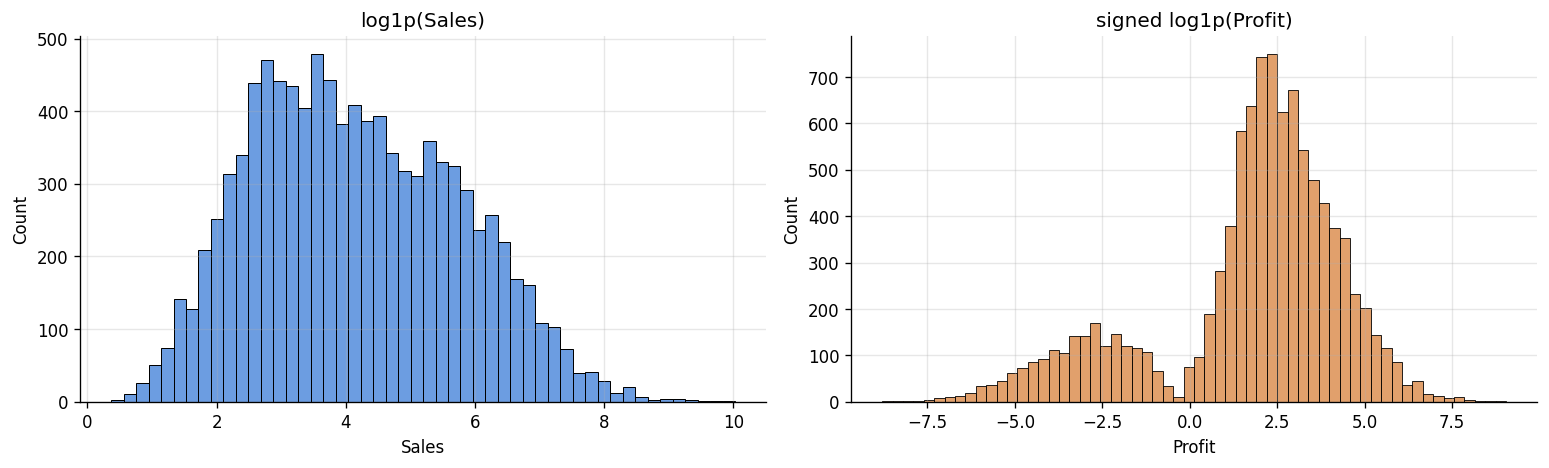
\includegraphics[width=0.95\linewidth]{02_log_transforms.png}
  \caption{Left: $\log(1+\text{Sales})$ recovers an approximately unimodal,
  near-symmetric shape (\cref{eq:skew} in the raw scale is large and
  positive; after the transform it is close to zero). Right: signed
  $\log(1+|\text{Profit}|)$, showing the loss-making mass as a distinct
  negative lobe rather than a long left tail.}
  \label{fig:log-dist}
\end{figure}

\begin{figure}[H]
  \centering
  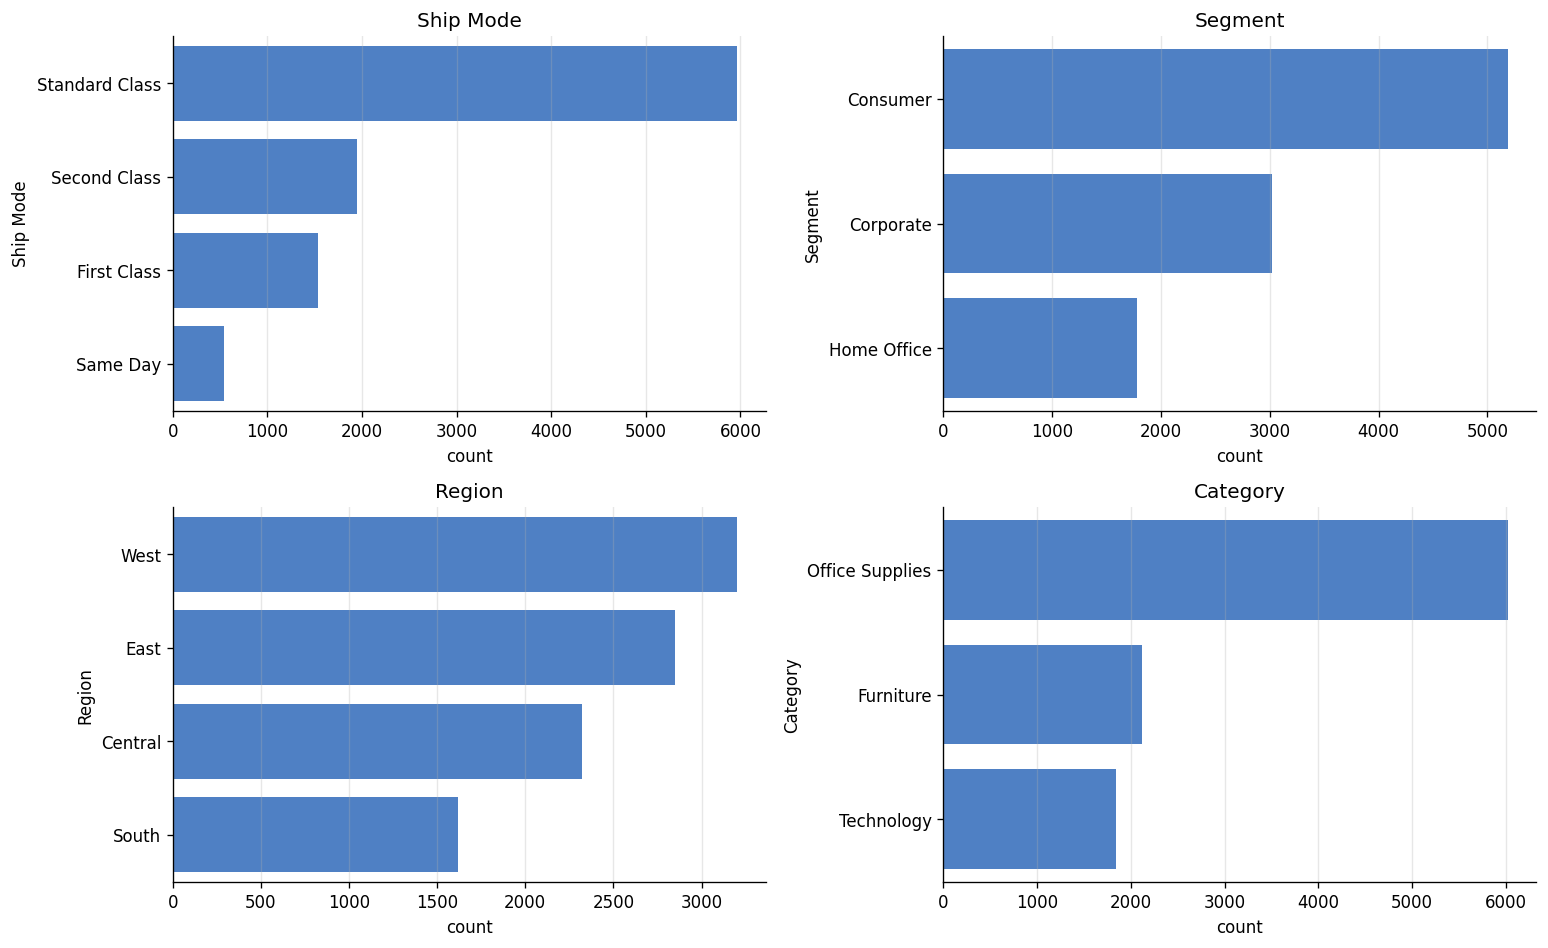
\includegraphics[width=0.95\linewidth]{02_univariate_categorical.png}
  \caption{Order-line counts by \texttt{Ship Mode}, \texttt{Segment},
  \texttt{Region} and \texttt{Category}. Standard Class and the Consumer
  segment dominate; the four regions are comparably sized, with West
  largest.}
  \label{fig:cat-dist}
\end{figure}

\subsection{Profit by product hierarchy}
Table~\ref{tab:subcat-profit} (full detail in
\texttt{outputs/tables/02\_by\_subcategory.csv}) aggregates profit by
sub-category. \textbf{Tables} lose \$17{,}725 overall despite \$207k of
sales, and \textbf{Bookcases} lose \$3{,}473 — both at average discounts
above 21\%, well above the store-wide mean. \textbf{Supplies} is also
marginally loss-making. Every other sub-category is net profitable, led by
Copiers (37\% margin) and Phones (\$330k sales, 13\% margin).

\begin{table}[H]
  \centering
  \caption{Selected sub-categories by total profit (ascending). Full table
  has all 17 sub-categories.}
  \label{tab:subcat-profit}
  \begin{tabular}{@{}llrrrr@{}}
    \toprule
    Category & Sub-Category & Sales (\$) & Profit (\$) & Avg.\ Discount & Margin \\
    \midrule
    Furniture & Tables      & 206{,}966 & $-$17{,}725 & 26.1\% & $-$8.6\% \\
    Furniture & Bookcases   & 114{,}880 & $-$3{,}473  & 21.1\% & $-$3.0\% \\
    Office Supplies & Supplies & 46{,}674 & $-$1{,}189 & 7.7\% & $-$2.5\% \\
    \multicolumn{6}{c}{\dots (14 profitable sub-categories) \dots} \\
    Technology & Phones     & 330{,}007 & 44{,}516    & 15.5\% & 13.5\% \\
    Technology & Copiers    & 149{,}528 & 55{,}618    & 16.2\% & \textbf{37.2\%} \\
    \bottomrule
  \end{tabular}
\end{table}

\begin{figure}[H]
  \centering
  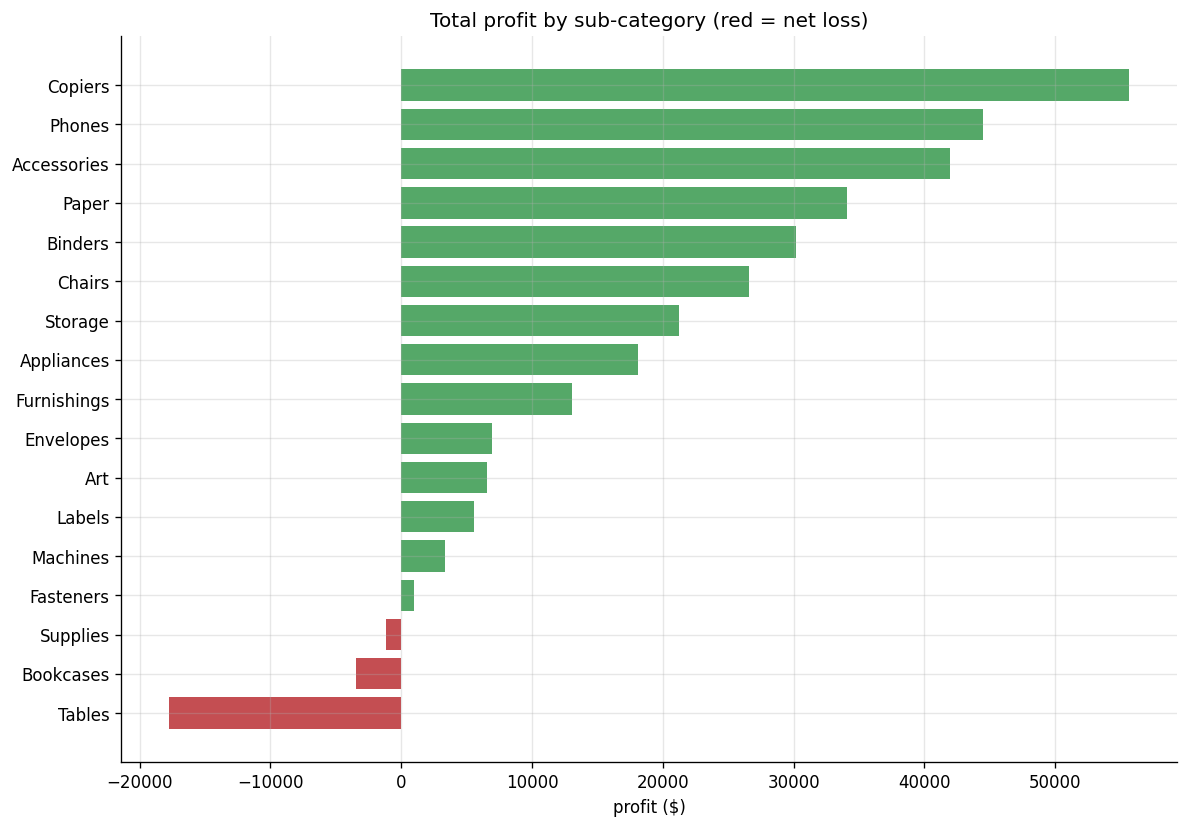
\includegraphics[width=0.8\linewidth]{02_profit_by_subcategory.png}
  \caption{Total profit by sub-category; red bars are net loss-makers.}
  \label{fig:subcat-profit}
\end{figure}

\begin{figure}[H]
  \centering
  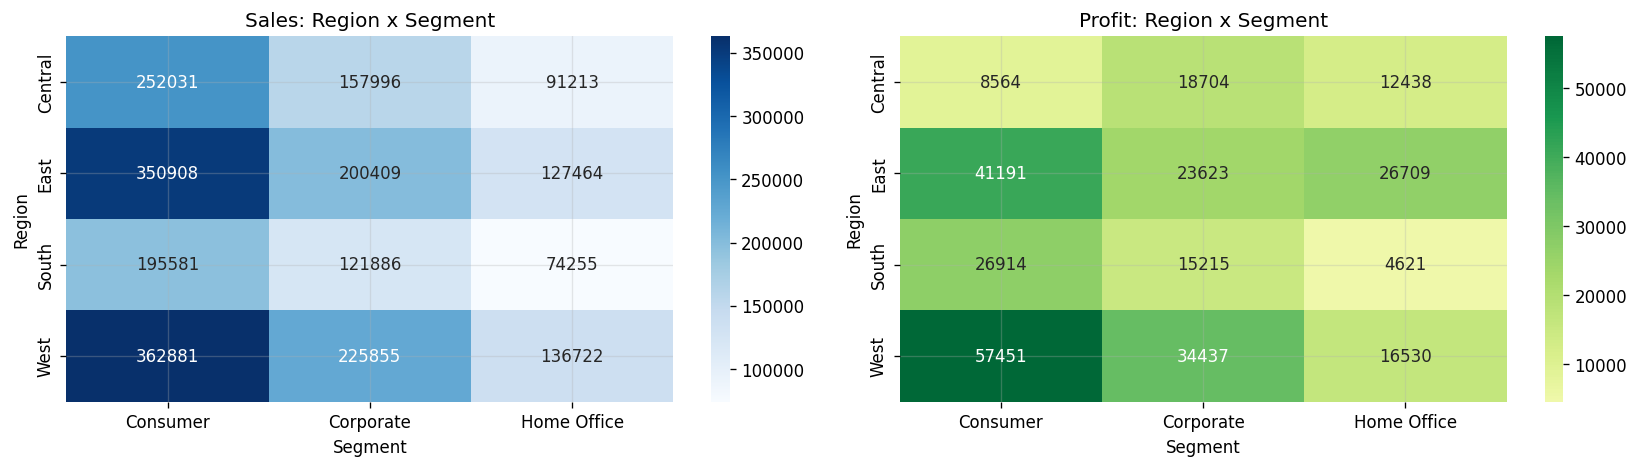
\includegraphics[width=0.85\linewidth]{02_region_segment_heatmap.png}
  \caption{Sales (left) and profit (right) cross-tabulated by Region and
  Segment. Sales are fairly even across cells; profit is not — the
  Central/Consumer cell is comparatively weak.}
  \label{fig:region-segment}
\end{figure}

\subsection{Discount versus profit}
\label{sec:eda-discount-profit}
\begin{figure}[H]
  \centering
  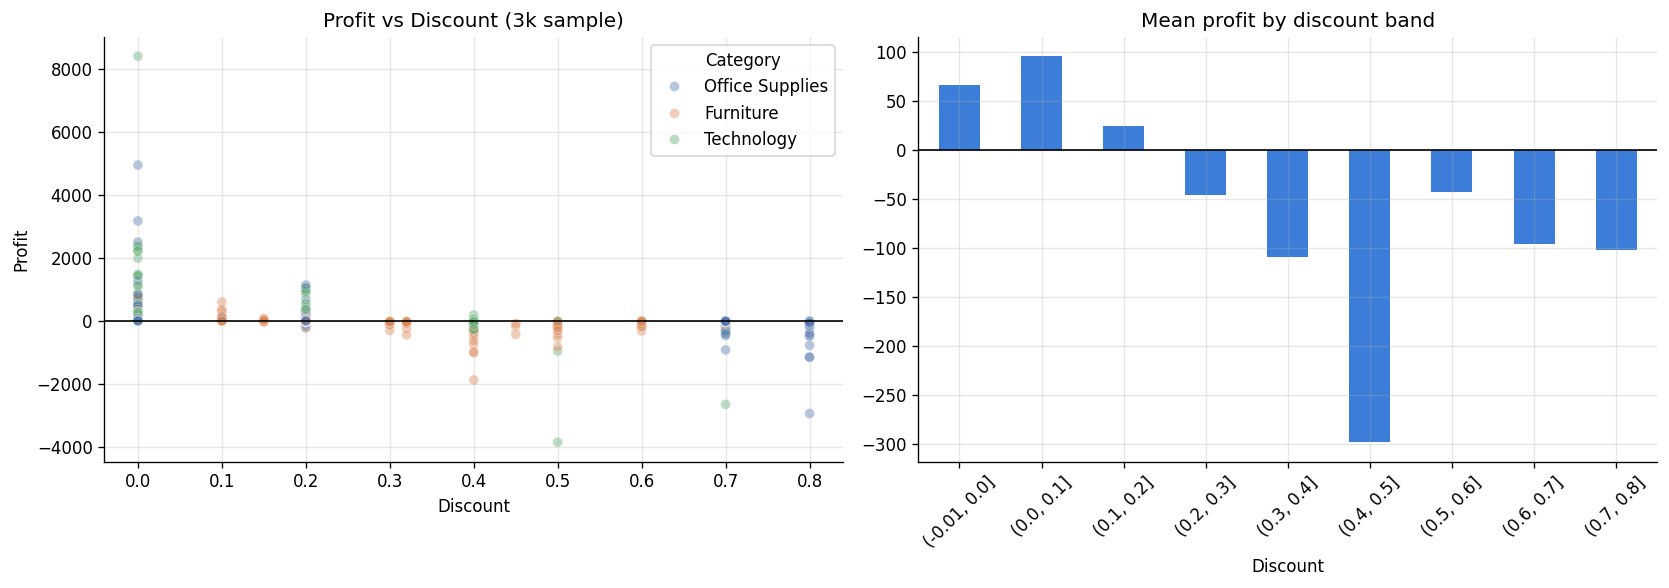
\includegraphics[width=0.95\linewidth]{02_discount_vs_profit.png}
  \caption{Left: line-level profit vs.\ discount (3,000-row sample),
  coloured by category — profit is scattered near zero at low discount and
  swings sharply negative as discount grows. Right: mean profit by
  discount band, crossing zero between the 10--20\% and 20--30\% bands and
  falling steeply beyond 30\%.}
  \label{fig:discount-profit}
\end{figure}
Quantitatively, the loss rate ($\Pr(\text{Profit}<0)$) is
\textbf{exactly 0\%} for undiscounted lines and \textbf{96.8\%} for lines
discounted 30\% or more, against an overall loss rate of 18.7\% across all
9{,}994 lines — discount depth is close to a deterministic switch, not a
mild risk factor. Because the relationship is a threshold
effect rather than linear, the raw Pearson correlation between
\texttt{Discount} and \texttt{Profit} (visible in
\cref{fig:corr-heatmap}) understates its practical importance; this
motivates using the categorical \texttt{discount\_bucket} feature (rather
than relying on a linear term alone) in \cref{ch:features,ch:models}.

\begin{figure}[H]
  \centering
  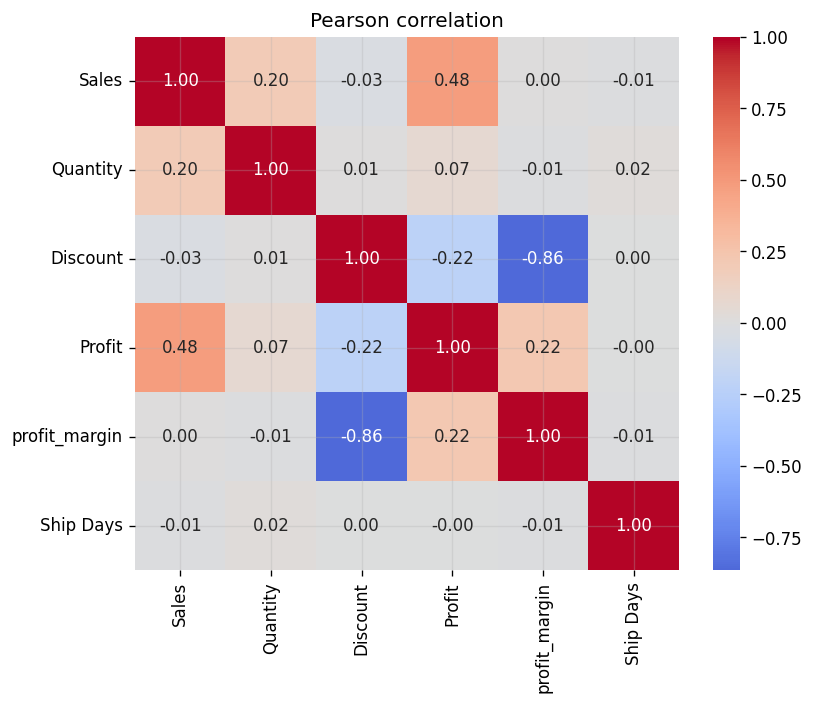
\includegraphics[width=0.55\linewidth]{02_correlation.png}
  \caption{Pearson correlation (\cref{eq:pearson}) among the core numeric
  fields. \texttt{Sales}--\texttt{Profit}: $\rho\approx0.48$;
  \texttt{Discount}--\texttt{Profit}: $\rho\approx-0.22$ (negative but,
  per \cref{fig:discount-profit}, understating the non-linear effect);
  \texttt{Quantity} is nearly uncorrelated with profit.}
  \label{fig:corr-heatmap}
\end{figure}

\subsection{Seasonality}
\begin{figure}[H]
  \centering
  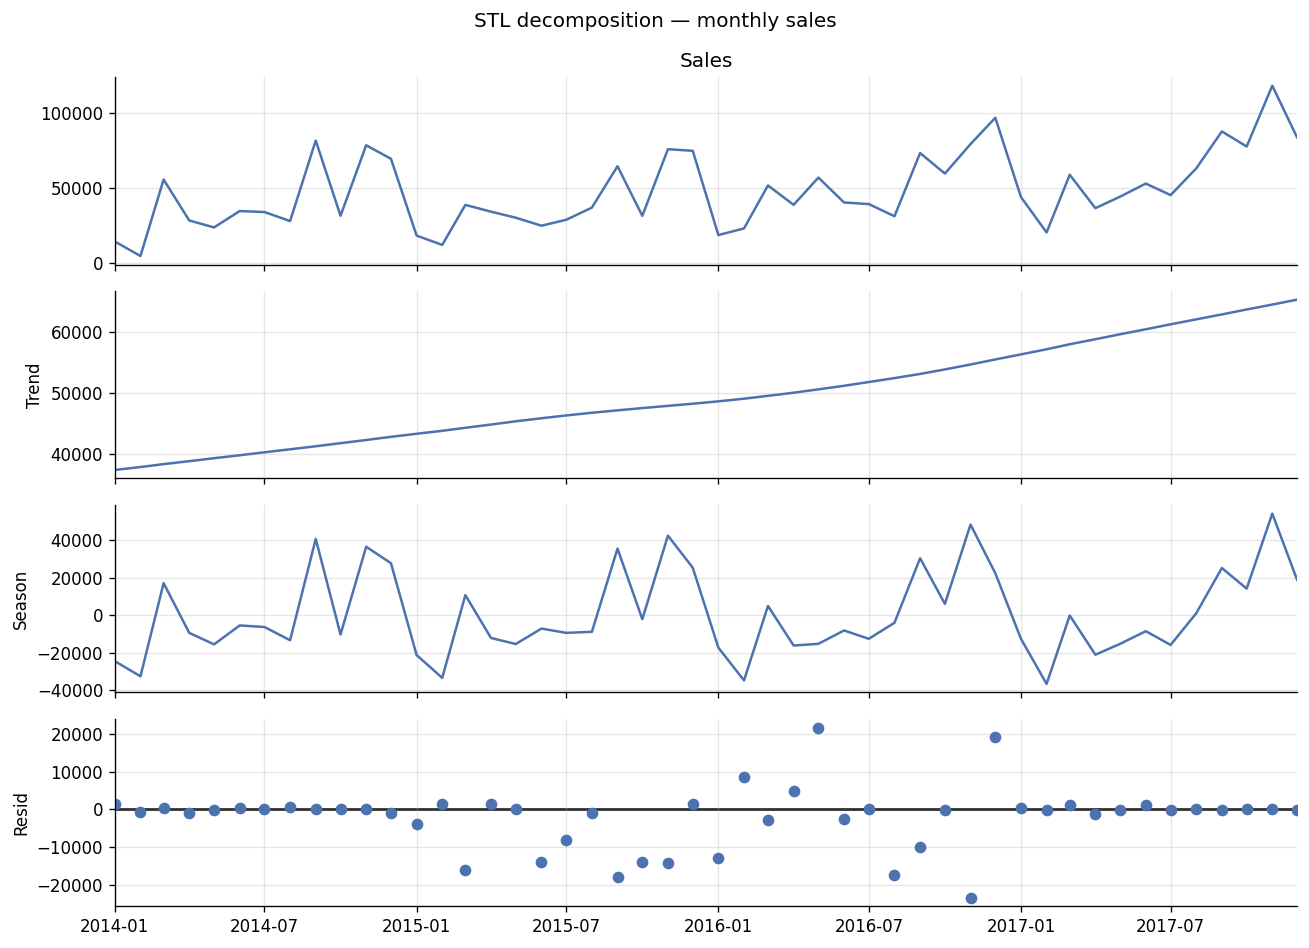
\includegraphics[width=0.95\linewidth]{02_stl_decomposition.png}
  \caption{STL decomposition (\cref{eq:stl-additive}, period 12) of monthly
  sales: a clear upward trend across the four years and a recurring
  within-year seasonal pattern that peaks late in the year, leaving a
  comparatively small, structure-free remainder.}
  \label{fig:stl}
\end{figure}
\begin{figure}[H]
  \centering
  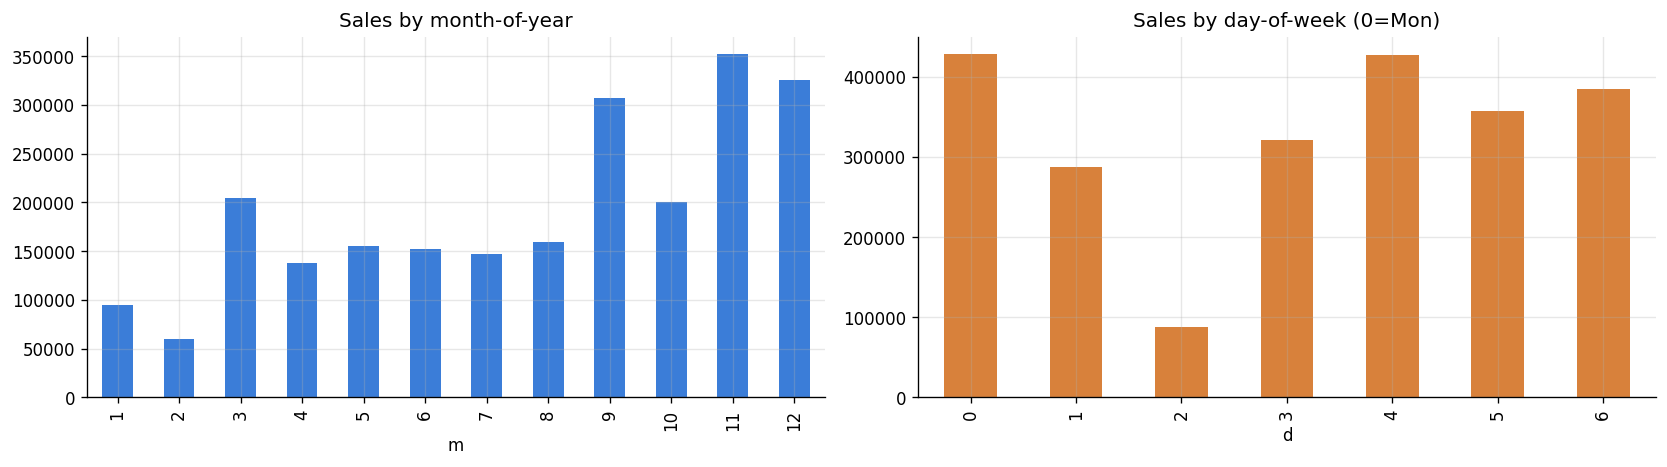
\includegraphics[width=0.95\linewidth]{02_seasonal_profiles.png}
  \caption{Sales aggregated by month-of-year (left) and day-of-week
  (right, 0 = Monday). November--December is by far the strongest period;
  day-of-week shows only mild variation.}
  \label{fig:seasonal-profiles}
\end{figure}

\subsection{Customers and products}
The top-10 customers by sales (Table~\ref{tab:top-cust}) generate between
\$12k and \$25k each, but profitability is uneven within that list —
\emph{Sean Miller} is the single largest customer by revenue (\$25{,}043)
yet is net loss-making ($-\$1{,}981$), while \emph{Tamara Chand} generates
comparable revenue at a much healthier margin. The same pattern repeats at
product level: the \emph{Cisco TelePresence System EX90} and two
\emph{GBC} binding systems are top-10 by revenue but net loss-making,
again tracing back to discount depth on high-ticket Technology and
Furniture items.

\begin{table}[H]
  \centering
  \caption{Top 5 customers by total sales.}
  \label{tab:top-cust}
  \begin{tabular}{@{}lrrr@{}}
    \toprule
    Customer & Sales (\$) & Profit (\$) & Orders \\
    \midrule
    Sean Miller     & 25{,}043 & $-$1{,}981 & 5 \\
    Tamara Chand    & 19{,}052 & 8{,}981    & 5 \\
    Raymond Buch    & 15{,}117 & 6{,}976    & 6 \\
    Tom Ashbrook    & 14{,}596 & 4{,}704    & 4 \\
    Adrian Barton   & 14{,}474 & 5{,}445    & 10 \\
    \bottomrule
  \end{tabular}
\end{table}

\section{Interpretation}
Three findings from this chapter shape every subsequent stage of the
report. First, the data requires \emph{no} missing-value or duplicate
handling, so all modelling error downstream is genuinely about the
signal, not data-cleaning artefacts. Second, \textbf{discount depth, not
category or region, is the primary lever on profitability} — a threshold
effect around 30\% discount that is far stronger than any single-variable
linear correlation suggests, which is why \texttt{discount\_bucket}
(\cref{ch:features}) and the corresponding permutation-importance results
(\cref{ch:models}) recur as the dominant signal throughout the rest of the
report. Third, the pronounced trend and December seasonality in
\cref{fig:stl} is exactly the structure a seasonal model must capture,
and directly motivates the choice of Holt-Winters and SARIMA — both
explicitly seasonal — over simpler alternatives in \cref{ch:forecasting}.

\chapter{Feature Engineering}
\label{ch:features}

\section{Theory}

\subsection{Data leakage}
\begin{definition}[Leakage]
A feature $x^{(j)}$ used to predict target $y_i$ for observation $i$
\emph{leaks} if it is constructed, even indirectly, from information that
would not be available at the moment a real prediction for $i$ has to be
made — most commonly, information from $i$'s own future or from $i$
itself when $y_i$ is a deterministic function of it.
\end{definition}
Leakage is the single most common cause of a model that performs
excellently offline and fails in production, because the leaked signal
is unavailable (or has a different distribution) at serving time. Two
concrete leakage risks are present in this dataset and are handled
explicitly:
\begin{enumerate}[label=(\alph*)]
  \item \textbf{Target leakage}: \texttt{profit\_margin} $=
        \text{Profit}/\text{Sales}$ is definitionally almost the target
        (\texttt{Profit}) rescaled, so it is computed only for exploratory
        plots (\cref{ch:eda}) and \emph{never} included in the supervised
        feature matrix $\mathbf{X}$.
  \item \textbf{Temporal leakage in customer aggregates}: a naive
        "customer's total historical sales" feature computed with a
        normal \texttt{groupby(...).sum()} would, for order $i$, include
        sales from orders placed \emph{after} $i$ — information a
        real-time system could not have. We instead compute, for
        customer $c$ and a chronologically ordered sequence of their
        orders $i_1 < i_2 < \dots$,
        \begin{equation}
          h_k = f\bigl(\{v_{i_1}, \dots, v_{i_{k-1}}\}\bigr), \qquad
          h_1 = f(\varnothing),
          \label{eq:expanding}
        \end{equation}
        i.e. an \emph{expanding window statistic shifted by one}, so
        $h_k$ (the feature attached to the $k$-th order) is a function
        only of the customer's strictly \emph{prior} orders. In
        \texttt{pandas} this is exactly
        \texttt{groupby(id)[col].apply(lambda s: s.shift().expanding().}
        \texttt{agg(f))}, and it is verified empirically in
        \cref{sec:feat-results} by checking that every customer's first
        order has a history of identically zero.
\end{enumerate}

\subsection{Cyclical (circular) encoding of periodic variables}
Calendar fields such as month-of-year $m \in \{1,\dots,12\}$ or
day-of-week $d\in\{0,\dots,6\}$ are \emph{circular}: December (12) is
adjacent to January (1), not maximally distant from it, yet a plain
integer encoding implies exactly that. Passing $m$ into a linear or
distance-based model as a raw integer therefore injects a false ordinal
distance. The standard fix is to embed the period on the unit circle,
\begin{equation}
  m_{\sin} = \sin\!\left(\frac{2\pi m}{12}\right), \qquad
  m_{\cos} = \cos\!\left(\frac{2\pi m}{12}\right),
  \label{eq:cyclical}
\end{equation}
so that the Euclidean distance between two months' encodings,
$\sqrt{(m_{\sin}-m'_{\sin})^2+(m_{\cos}-m'_{\cos})^2} =
2\left|\sin\frac{\pi(m-m')}{12}\right|$, is a monotone function of their
true circular distance and wraps correctly around the year boundary.
Tree ensembles (used for the best-performing models in
\cref{ch:models,ch:forecasting}) do not strictly require this — they can
split $m$ arbitrarily and effectively rediscover adjacency — but linear
and distance-based components still benefit, and the encoding is cheap
and included uniformly.

\subsection{Categorical encoding}
For a categorical field with levels $\{c_1,\dots,c_K\}$, \emph{one-hot
encoding} maps a value $c_k$ to the $k$-th standard basis vector
$\mathbf{e}_k \in \{0,1\}^K$, avoiding the false ordinal structure that
a plain integer code would impose on an unordered category, at the cost
of adding $K-1$ columns (one level dropped or absorbed as the reference
via collinearity handling). With $K$ large or with many rare levels — the
Superstore data has 49 U.S. states, most with a handful of orders — this
inflates dimensionality and lets a model overfit to noise in
low-count categories. We mitigate this by collapsing any level occurring
fewer than 20 times into a single \texttt{"infrequent"} bucket before
one-hot expansion (scikit-learn's \texttt{OneHotEncoder(min\_frequency=}
\texttt{20)}), trading a small amount of resolution for materially lower
variance in the corresponding coefficient/split estimates.

\subsection{RFM analysis}
\textbf{RFM} (Recency, Frequency, Monetary) is a classical customer
segmentation heuristic from direct-marketing analytics. For customer $c$
and an analysis snapshot date $\tau$,
\begin{align}
  R_c &= \tau - \max\{\text{Order Date} : \text{orders of } c\}, \\
  F_c &= \bigl|\{\text{distinct orders of } c\}\bigr|, \\
  M_c &= \sum_{\text{orders of } c} \text{Sales}.
\end{align}
Each of $R$, $F$, $M$ is independently discretised into quintiles
(1 = worst, 5 = best; $R$ is inverted since \emph{smaller} recency is
better), and an overall score $\mathrm{RFM}_c = r_c+f_c+m_c \in [3,15]$
ranks customers by a simple, interpretable combination of how recently,
how often, and how much they buy — used here purely as a descriptive
segmentation (\cref{sec:feat-results}), not as a model feature (to avoid
mixing a snapshot-time construct into the leakage-safe, per-order feature
matrix).

\subsection{Right-skew and the log transform, revisited}
As introduced in \cref{ch:eda}, $\log(1+x)$ is applied to \texttt{Sales}
as an explicit feature (\texttt{log\_sales}) rather than only a plotting
device, because linear/coefficient-based models benefit from the reduced
skew and more homoscedastic residual structure it induces, while the
tree-based models used in \cref{ch:models} are monotone-transform
invariant and are unaffected by whether it is present.

\section{Method}
All logic lives in \texttt{src/features.py} and is exercised end to end
in \texttt{03\_feature\_engineering.ipynb}. \texttt{add\_targets} derives
\texttt{profit\_margin} and \texttt{is\_loss} (kept out of $\mathbf{X}$
as above); \texttt{add\_date\_features} derives calendar parts and the
sin/cos pairs of \cref{eq:cyclical}; \texttt{add\_line\_features} derives
\texttt{price\_per\_unit}, \texttt{log\_sales}, \texttt{is\_discounted},
and a 5-level \texttt{discount\_bucket} (\emph{none / low / mid / high /
extreme}, edges at 0, 15\%, 30\%, 50\%); \texttt{add\_customer\_history}
implements the expanding-shift computation of \cref{eq:expanding} for
prior order count, prior sales sum/mean, prior loss rate, and days since
the customer's first order. \texttt{make\_supervised} assembles the final
$n\times p$ matrix $\mathbf{X}$ (26 numeric + 6 categorical columns,
categoricals left as raw strings for the modelling pipeline's own
\texttt{OneHotEncoder} in \cref{ch:models}) and the two targets
$\mathbf{y}_{\text{reg}}=\text{Profit}$, $\mathbf{y}_{\text{clf}}=
\text{is\_loss}$.

\section{Results}
\label{sec:feat-results}

\subsection{Feature matrix and leakage check}
Building the full feature frame adds 26 engineered columns to the 21 raw
ones, and the final supervised matrix is $\mathbf{X}\in
\mathbb{R}^{9994\times 32}$ with \textbf{zero missing values}. The
leakage sanity check passes exactly as designed: across all 793
customers' first-ever order line, \texttt{cust\_prior\_lines} and
\texttt{cust\_prior\_sales\_sum} are identically 0 — no customer's first
transaction sees any of their own future purchase history.

\begin{figure}[H]
  \centering
  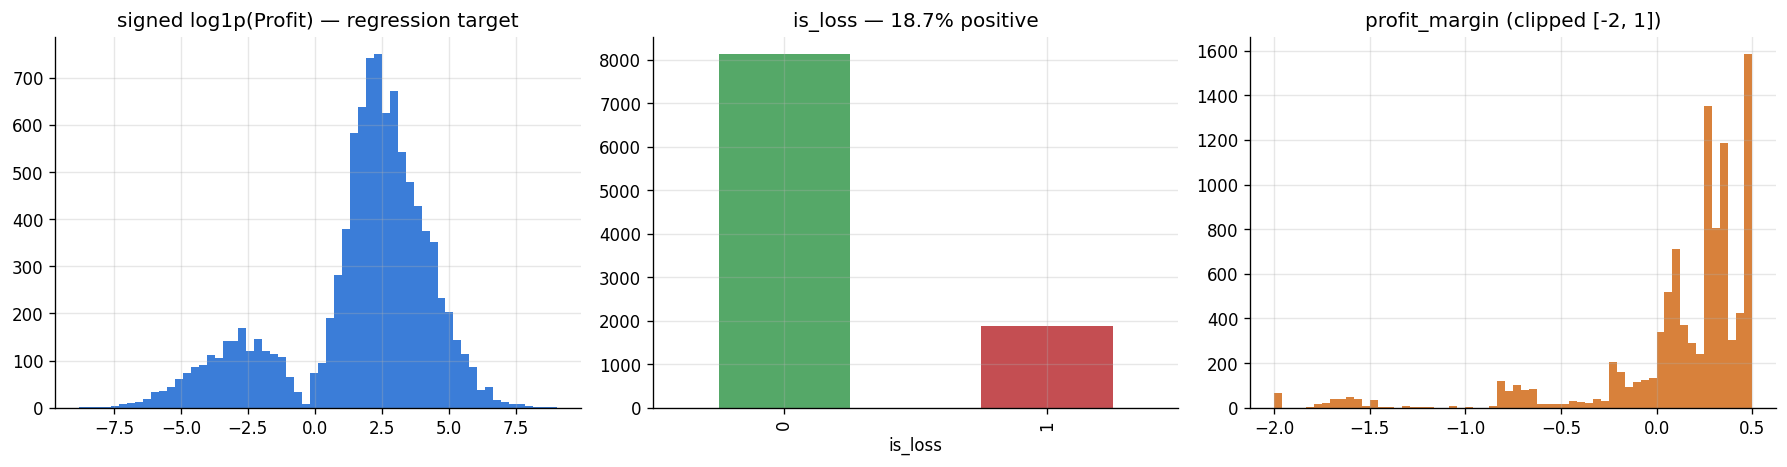
\includegraphics[width=0.95\linewidth]{03_targets.png}
  \caption{The two supervised targets and the exploratory \texttt{profit\_margin}: signed
  log-profit (left), the binary \texttt{is\_loss} class balance — 18.7\%
  positive (middle), and margin distribution (right).}
  \label{fig:feat-targets}
\end{figure}

\begin{figure}[H]
  \centering
  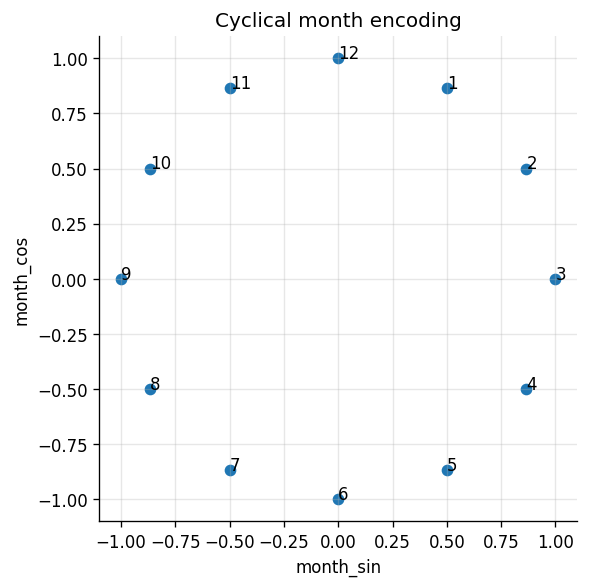
\includegraphics[width=0.55\linewidth]{03_cyclical_month.png}
  \caption{The 12 months placed on the unit circle by
  \cref{eq:cyclical}: December and January are adjacent, as they should
  be, unlike under a raw integer encoding.}
  \label{fig:feat-cyclical}
\end{figure}

\subsection{Discount buckets}
Table~\ref{tab:discount-bucket} operationalises the threshold effect
found in \cref{ch:eda}: mean profit and loss rate degrade monotonically
across buckets, flipping sign between \emph{mid} and \emph{high}, and the
\emph{extreme} bucket (discount $\geq 50\%$) is loss-making on
\textbf{every single line} in the data.

\begin{table}[H]
  \centering
  \caption{Line-level statistics by \texttt{discount\_bucket}.}
  \label{tab:discount-bucket}
  \begin{tabular}{@{}lrrrr@{}}
    \toprule
    Bucket & $n$ & Mean profit (\$) & Loss rate & Mean margin \\
    \midrule
    none (0\%)        & 4{,}798 & 66.90   & 0.0\%   & 34.0\% \\
    low (0--15\%)      & 146     & 71.56   & 14.4\%  & 11.2\% \\
    mid (15--30\%)     & 3{,}884 & 20.59   & 18.3\%  & 16.0\% \\
    high (30--50\%)    & 310     & $-$156.28 & 91.6\% & $-$29.6\% \\
    extreme ($\geq$50\%) & 856   & $-$89.44  & \textbf{100.0\%} & $-$113.9\% \\
    \bottomrule
  \end{tabular}
\end{table}

\subsection{Customer history features}
\begin{figure}[H]
  \centering
  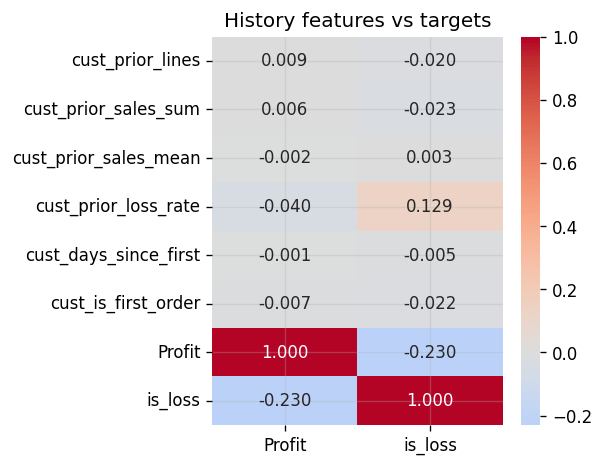
\includegraphics[width=0.55\linewidth]{03_history_vs_target.png}
  \caption{Correlation of the leakage-safe customer-history features with
  the two targets. \texttt{cust\_prior\_loss\_rate} is the strongest of
  the six ($\rho=0.129$ with \texttt{is\_loss}) — a customer who has
  previously bought at deep discounts is more likely to do so again.}
  \label{fig:feat-history-corr}
\end{figure}
The other history features (prior line count, prior sales sum/mean, days
since first order) correlate only weakly ($|\rho| < 0.03$) with either
target at the line level — unsurprising, since a given customer's
profit outcome on \emph{this} line is driven mostly by \emph{this}
line's own discount, not by how much they have historically spent.

\subsection{RFM segmentation}
\begin{figure}[H]
  \centering
  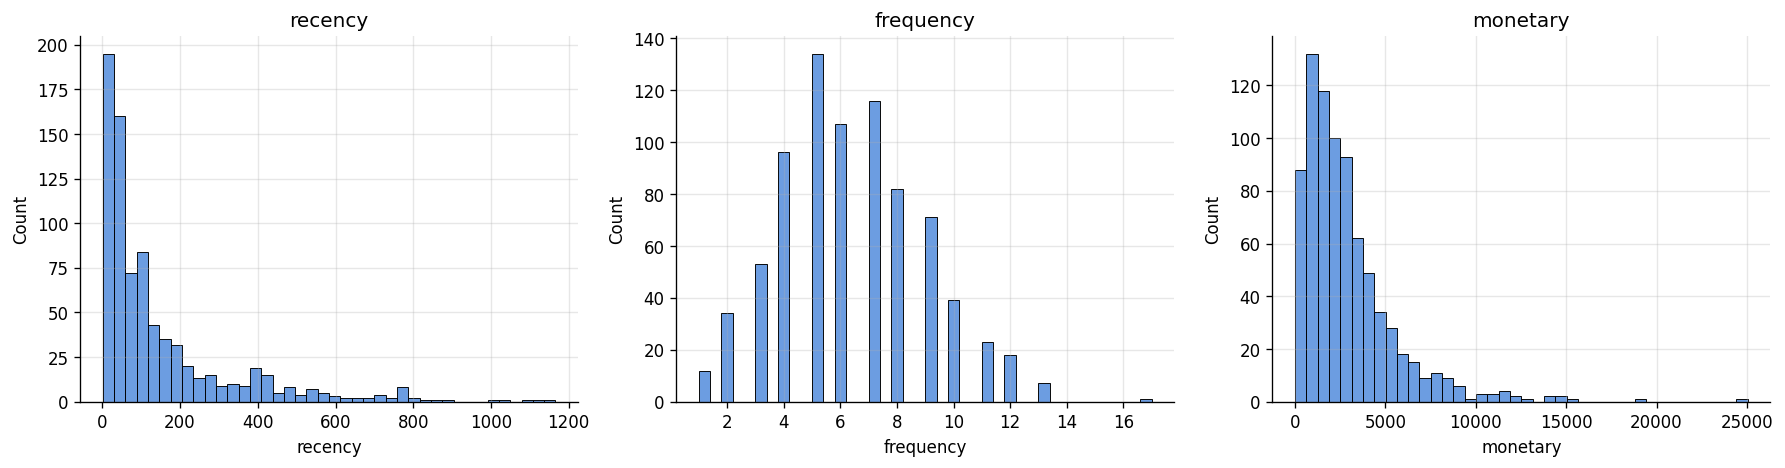
\includegraphics[width=0.95\linewidth]{03_rfm_distributions.png}
  \caption{Distributions of Recency, Frequency and Monetary value across
  the 793 customers.}
  \label{fig:feat-rfm-dist}
\end{figure}

\begin{table}[H]
  \centering
  \caption{RFM segments (score bands on $R+F+M \in[3,15]$).}
  \label{tab:rfm-segments}
  \begin{tabular}{@{}lrrrr@{}}
    \toprule
    Segment & Customers & Avg.\ Monetary (\$) & Avg.\ Frequency & Avg.\ Recency (days) \\
    \midrule
    At risk           & 196 & 989   & 3.7 & 329 \\
    Needs attention    & 219 & 2{,}160 & 5.6 & 138 \\
    Loyal              & 254 & 3{,}869 & 7.4 & 75 \\
    Champions          & 124 & 5{,}221 & 9.4 & 28 \\
    \bottomrule
  \end{tabular}
\end{table}
The four segments form a coherent gradient: Champions buy 2.5$\times$ more
often and spend 5.3$\times$ more per customer on average than the
At-risk segment, and were last seen 12$\times$ more recently — exactly
the monotone structure RFM is designed to expose.

\section{Interpretation}
The leakage-safe construction of the customer-history features is the
methodologically important result of this chapter: it guarantees that the
2017 hold-out evaluation in \cref{ch:models} is a fair test of
generalisation to a genuinely unseen future, not an artefact of features
that implicitly encode the answer. Substantively, the discount-bucket
table makes the EDA finding operational and almost mechanical:
\emph{extreme} discounting is loss-making with effective certainty in
this dataset, which is precisely the signal the classifier of
\cref{ch:models} is able to exploit to reach a PR-AUC of 0.96. RFM
segmentation, while not fed into the predictive models, gives an
independent, interpretable customer lens that a retail analytics team
could pair with the profit/loss model output — e.g. prioritising discount
governance on At-risk/Needs-attention customers, where a marginal loss
is more likely to also coincide with a customer who is not being
retained by it anyway.

\chapter{Forecasting Monthly Sales}
\label{ch:forecasting}

This is the most theory-heavy chapter of the report: forecasting a short
(48-point) monthly series correctly requires care about stationarity,
model identification, and — critically — an evaluation protocol that
respects time order, none of which arise in the i.i.d.\ supervised setting
of \cref{ch:models}.

\section{Theory}

\subsection{Stationarity}
\begin{definition}[Weak stationarity]
A process $\{y_t\}$ is \emph{weakly (covariance) stationary} if
$\mathbb{E}[y_t] = \mu$ is constant in $t$, $\mathrm{Var}(y_t)=\sigma^2$
is constant in $t$, and $\mathrm{Cov}(y_t, y_{t+h})$ depends on the lag
$h$ but not on $t$ itself.
\end{definition}
Classical linear time-series models (AR, MA, ARMA) are defined for
stationary processes; a series with a trend or a growing seasonal
amplitude violates the definition and must be transformed — typically by
\emph{differencing} — before such a model applies. The backshift (lag)
operator $B$, $By_t = y_{t-1}$, lets a $d$-th order difference be written
compactly as $\Delta^d y_t = (1-B)^d y_t$; a \emph{seasonal} difference of
period $s$ is $\Delta_s y_t = (1-B^s) y_t = y_t - y_{t-s}$.

\subsection{The augmented Dickey--Fuller test}
The ADF test formalises "does this series need differencing" as a
hypothesis test on the regression
\begin{equation}
  \Delta y_t = \alpha + \beta t + \gamma y_{t-1}
             + \sum_{i=1}^{k}\delta_i \Delta y_{t-i} + \varepsilon_t,
  \label{eq:adf}
\end{equation}
with null hypothesis $H_0: \gamma = 0$ (a unit root — the series is a
random walk, non-stationary) against $H_1: \gamma < 0$ (stationary). The
test statistic is the ordinary $t$-statistic for $\hat\gamma$, but its
null distribution is \emph{not} the usual Student-$t$ (it is skewed left
by the non-standard behaviour of a random walk's sample variance), so
Dickey and Fuller's own tabulated critical values (or the software's
$p$-value approximation) must be used rather than a normal-theory table.

\subsection{Autocorrelation and the Box--Jenkins identification}
The autocorrelation function $\rho(h) = \mathrm{Corr}(y_t, y_{t+h})$ and
partial autocorrelation function $\phi_{hh}$ (the correlation between
$y_t$ and $y_{t+h}$ after regressing out $y_{t+1},\dots,y_{t+h-1}$) are
the classical diagnostic pair for identifying ARMA order: an AR($p$)
process has a PACF that cuts off after lag $p$ and an ACF that decays
geometrically, while an MA($q$) process has the mirror-image behaviour.
In practice for a short, strongly seasonal series like ours, ACF/PACF are
used qualitatively (\cref{fig:fc-acf-pacf}) to corroborate, not to
mechanically dictate, the model order.

\subsection{Exponential smoothing (Holt--Winters)}
Simple exponential smoothing forecasts the next value as a
geometrically-weighted average of the past, $\hat y_{t+1} = \alpha y_t +
(1-\alpha)\hat y_t$. \textbf{Holt--Winters} extends this with a trend
state $b_t$ and a seasonal state $s_t$ (period $L=12$). The additive
form used here is
\begin{align}
  \ell_t &= \alpha (y_t - s_{t-L}) + (1-\alpha)(\ell_{t-1}+b_{t-1}), \label{eq:hw-level}\\
  b_t &= \beta (\ell_t - \ell_{t-1}) + (1-\beta) b_{t-1}, \label{eq:hw-trend}\\
  s_t &= \gamma (y_t - \ell_t) + (1-\gamma) s_{t-L}, \label{eq:hw-season}\\
  \hat y_{t+h} &= \ell_t + h\,b_t + s_{t-L+((h-1)\bmod L)+1}, \label{eq:hw-forecast}
\end{align}
with smoothing parameters $\alpha,\beta,\gamma \in [0,1]$ chosen (by the
fitting routine) to minimise the in-sample sum of squared one-step
forecast errors. Level $\ell_t$ tracks the de-seasonalised local mean,
$b_t$ the local trend, and $s_t$ a smoothly-updating length-$L$ seasonal
profile; the $h$-step forecast \cref{eq:hw-forecast} linearly extrapolates
the trend and re-applies the appropriate seasonal index. This additive
form is appropriate when the seasonal swing has roughly constant absolute
size rather than growing proportionally with the level (a multiplicative
alternative replaces the $+s$ terms with $\times s$ terms), consistent
with \cref{fig:stl} where the seasonal amplitude does not visibly balloon
with the trend.

\subsection{SARIMA}
A seasonal ARIMA model, $\mathrm{SARIMA}(p,d,q)(P,D,Q)_s$, generalises
ARMA by combining non-seasonal and seasonal autoregressive/moving-average
polynomials applied to a series differenced both regularly ($d$ times)
and seasonally ($D$ times, period $s$):
\begin{equation}
  \phi_p(B)\,\Phi_P(B^s)\, (1-B)^d (1-B^s)^D y_t
    = \theta_q(B)\,\Theta_Q(B^s)\,\varepsilon_t,
  \label{eq:sarima}
\end{equation}
where $\phi_p(B) = 1-\phi_1 B - \cdots - \phi_p B^p$ (and analogously
$\Phi_P$, $\theta_q$, $\Theta_Q$ for the seasonal AR, non-seasonal MA and
seasonal MA polynomials respectively) and $\varepsilon_t$ is white noise.
We fit $\mathrm{SARIMA}(1,1,1)(1,1,0,12)$: one non-seasonal AR and MA
term, one seasonal AR term, one regular and one seasonal (period-12)
difference, and no seasonal MA term — a compact specification chosen to
be identifiable on 48 points while still capturing both the trend
($d=1$) and the year-over-year seasonal shape ($D=1$, period 12) directly,
rather than relying on Holt--Winters' exponential-smoothing-style
seasonal update. Coefficients are estimated by (quasi-)maximum likelihood
via the Kalman filter (as implemented in \texttt{statsmodels}'s
state-space \texttt{SARIMAX}), which also yields exact prediction
variances and hence analytic confidence intervals for the forecast.

\subsection{Forecast accuracy metrics}
For actuals $y_1,\dots,y_h$ and forecasts $\hat y_1,\dots,\hat y_h$ over a
horizon of length $h$:
\begin{align}
  \mathrm{MAE} &= \frac1h\sum_{i=1}^h |y_i - \hat y_i|, &
  \mathrm{RMSE} &= \sqrt{\frac1h\sum_{i=1}^h (y_i-\hat y_i)^2}, \\
  \mathrm{MAPE} &= \frac{100\%}{h}\sum_{i=1}^h \left|\frac{y_i-\hat y_i}{y_i}\right|. &&
\end{align}
MAE is in the original (dollar) units and treats all errors linearly;
RMSE is also in dollars but penalises large errors quadratically, so it
is more sensitive to occasional big misses (e.g. an under-forecast
December); MAPE is scale-free and hence comparable across series of
different magnitude (used here to compare the whole-store series against
per-category series of very different size), at the cost of being
undefined/unstable when $y_i$ is near zero and of asymmetrically
penalising over- vs.\ under-forecasts.

\subsection{Rolling-origin (walk-forward) backtesting}
A single train/test split, as used for the i.i.d.\ models of
\cref{ch:models}, is a poor evaluation protocol for a 48-point time
series: it tests the model at exactly one forecast origin, so its score
has high variance and cannot be trusted to represent typical future
performance. \textbf{Rolling-origin} (a.k.a.\ walk-forward, or expanding-
window) backtesting instead repeats the fit/forecast cycle at multiple
origins $o_1 < o_2 < \dots < o_K$: at each $o_k$, the model is trained
only on $y_1,\dots,y_{o_k}$ and scored against the next $h$ true values
$y_{o_k+1},\dots,y_{o_k+h}$, and the reported metric is the average
across the $K$ folds. This never trains on the future relative to any
fold's own test window and is the time-series analogue of $K$-fold
cross-validation, with the essential difference that folds must respect
temporal order rather than being drawn at random.

\subsection{Residual whiteness: the Ljung--Box test}
A well-specified model should leave residuals $\hat\varepsilon_t$ that
are approximately white noise (no remaining autocorrelation to exploit).
The Ljung--Box statistic
\begin{equation}
  Q_{LB} = n(n+2)\sum_{k=1}^{K}\frac{\hat\rho_k^2}{n-k}
  \label{eq:ljungbox}
\end{equation}
(with $\hat\rho_k$ the residual sample autocorrelation at lag $k$)
is asymptotically $\chi^2_K$ under the null of no autocorrelation up to
lag $K$; a large $p$-value (failure to reject) is the desired outcome,
indicating the model has not left exploitable structure behind.

\section{Method}
The monthly series $y_t = \sum_{\text{lines in month } t} \text{Sales}$
(\texttt{src.features.monthly\_sales}) has $T=48$ points, 2014-01 through
2017-12. We hold out the last 12 months as a single test window, fit
four forecasters on the code interface \texttt{fit(train)} /
\texttt{predict(h)} (\texttt{src/forecasting.py}) — a seasonal-naive
baseline, additive Holt--Winters, $\mathrm{SARIMA}(1,1,1)(1,1,0,12)$, and
a recursive random-forest regressor on lag/rolling-mean/seasonal features
(\texttt{LagRegressor}) — and separately run an 8-fold rolling-origin
backtest (\texttt{min\_train}=24, horizon=3, step=3). The winning point
forecaster is then refit on the full 48 months and projected 12 months
ahead; SARIMA additionally supplies an 80\% analytic confidence band via
its Kalman-filter forecast variance.

\section{Results}

\subsection{Series and stationarity}
\begin{figure}[H]
  \centering
  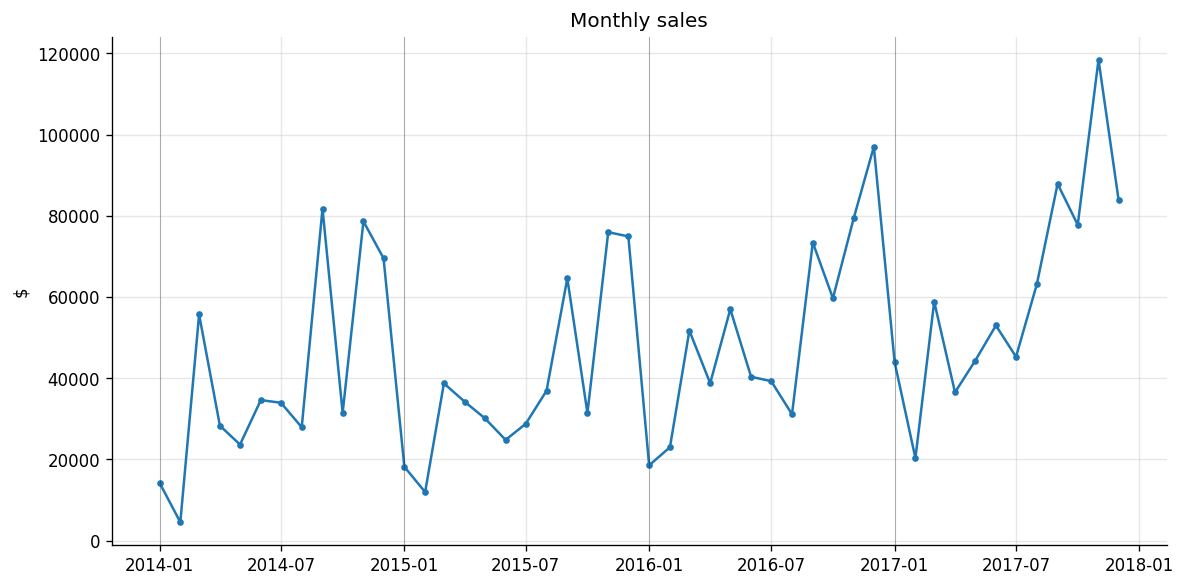
\includegraphics[width=0.95\linewidth]{04_series.png}
  \caption{Monthly sales, 2014--2017. Clear multi-year growth and a
  recurring within-year cycle.}
  \label{fig:fc-series}
\end{figure}
Table~\ref{tab:adf} reports the ADF test (\cref{eq:adf}) on the level
series, its first difference, and its seasonal (lag-12) difference.
\begin{table}[H]
  \centering
  \caption{ADF unit-root test, $H_0$: series has a unit root.}
  \label{tab:adf}
  \begin{tabular}{@{}lrr@{}}
    \toprule
    Series & Test statistic & $p$-value \\
    \midrule
    Level $y_t$                  & $-4.494$ & 0.0002 \\
    First difference $\Delta y_t$ & $-9.058$ & $<$0.0001 \\
    Seasonal difference $\Delta_{12} y_t$ & $-1.482$ & 0.5425 \\
    \bottomrule
  \end{tabular}
\end{table}
The level series already rejects a pure unit root, and first-differencing
rejects it far more decisively — but the \emph{seasonal-only} difference
does \textbf{not} (p = 0.54): removing only the year-over-year level
shift is not enough to leave a stationary residual, because the
within-year \emph{shape} of the cycle (not just its level) still carries
structure. This is exactly the case for using a model with an explicit,
separately-estimated seasonal component — Holt--Winters' $s_t$ state, or
SARIMA's combined regular-\emph{and}-seasonal differencing
(\cref{eq:sarima}, $d{=}1,D{=}1$) — rather than relying on a single
seasonal difference alone.
\begin{figure}[H]
  \centering
  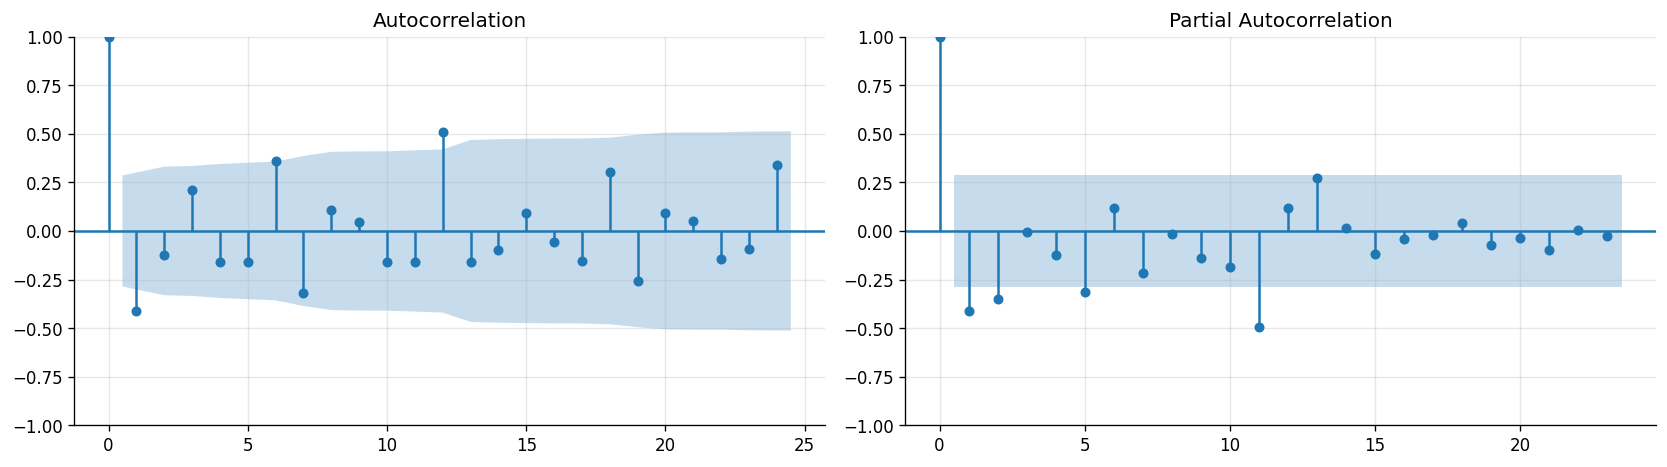
\includegraphics[width=0.95\linewidth]{04_acf_pacf.png}
  \caption{ACF (left) and PACF (right) of $\Delta y_t$. A significant
  spike near lag 12 in both is consistent with the seasonal structure
  seen directly in \cref{fig:fc-series,fig:stl}.}
  \label{fig:fc-acf-pacf}
\end{figure}

\subsection{Hold-out comparison}
\begin{table}[H]
  \centering
  \caption{12-month hold-out accuracy (train on months 1--36, test on 37--48).}
  \label{tab:holdout}
  \begin{tabular}{@{}lrrr@{}}
    \toprule
    Model & MAE (\$) & RMSE (\$) & MAPE \\
    \midrule
    \textbf{Holt--Winters} & \textbf{11{,}456} & 12{,}544 & \textbf{22.6\%} \\
    SARIMA(1,1,1)(1,1,0,12) & 13{,}411 & 15{,}989 & 26.7\% \\
    Lag-regressor (RF)      & 13{,}484 & 16{,}791 & 24.1\% \\
    Seasonal-naive baseline & 15{,}468 & 18{,}986 & 24.5\% \\
    \bottomrule
  \end{tabular}
\end{table}
\begin{figure}[H]
  \centering
  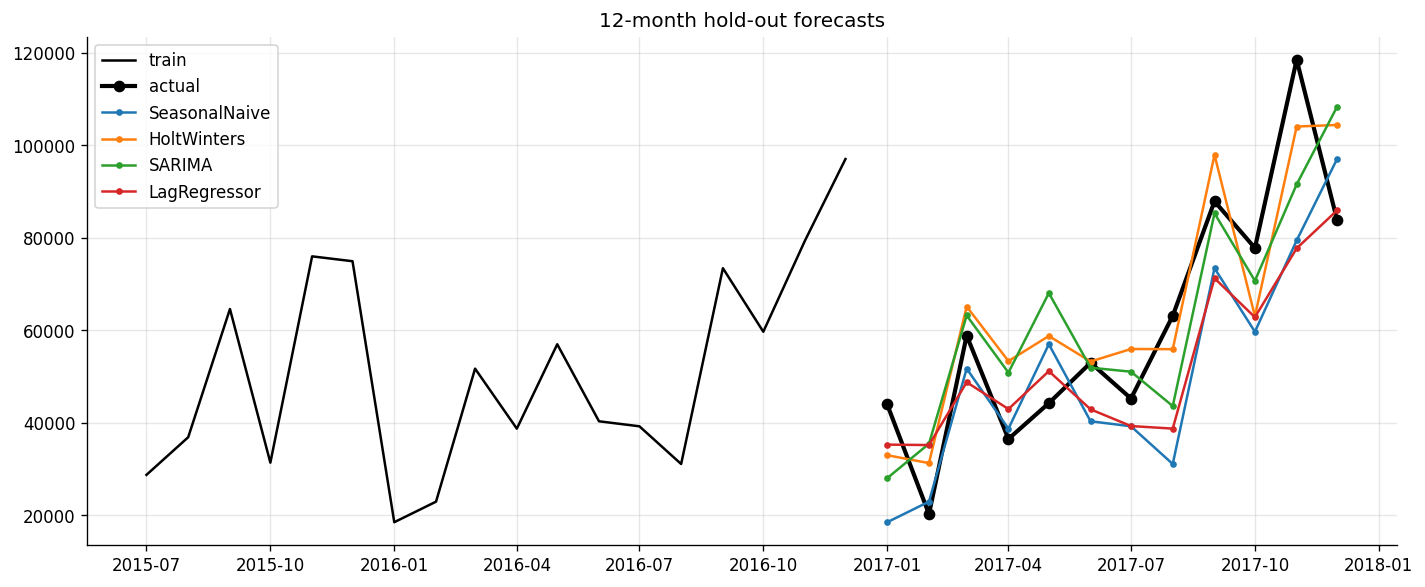
\includegraphics[width=0.95\linewidth]{04_holdout_forecasts.png}
  \caption{12-month hold-out: all four models' forecasts against the
  realised sales path.}
  \label{fig:fc-holdout}
\end{figure}
All three fitted models beat the seasonal-naive baseline on MAE and RMSE;
Holt--Winters is the clear winner on this single split.

\subsection{Rolling-origin backtest}
\begin{table}[H]
  \centering
  \caption{8-fold rolling-origin backtest (\texttt{min\_train}=24,
  horizon=3, step=3), metrics averaged across folds.}
  \label{tab:backtest}
  \begin{tabular}{@{}lrrrr@{}}
    \toprule
    Model & MAE (\$) & RMSE (\$) & MAPE & Folds \\
    \midrule
    \textbf{SARIMA}         & \textbf{11{,}612} & 13{,}373 & 23.9\% & 8 \\
    Holt--Winters            & 12{,}314 & 14{,}104 & 25.1\% & 8 \\
    Lag-regressor (RF)       & 13{,}660 & 15{,}527 & 27.2\% & 8 \\
    Seasonal-naive baseline  & 13{,}994 & 16{,}207 & 24.9\% & 8 \\
    \bottomrule
  \end{tabular}
\end{table}
\begin{figure}[H]
  \centering
  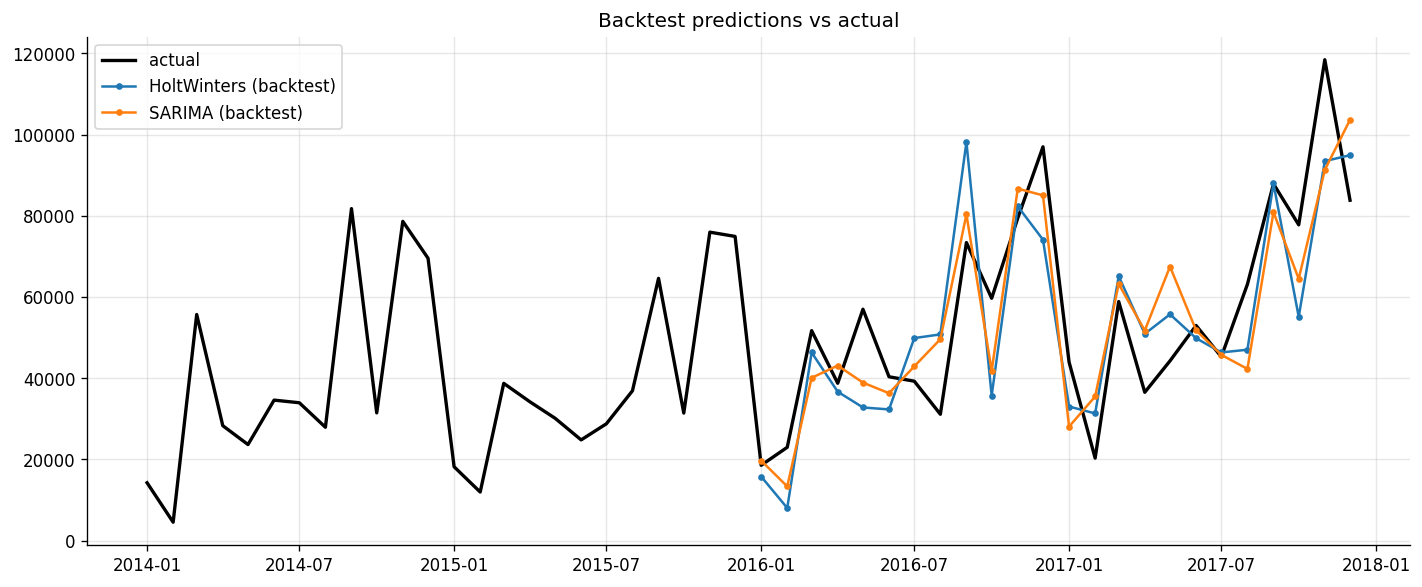
\includegraphics[width=0.95\linewidth]{04_backtest_predictions.png}
  \caption{Rolling-origin backtest predictions (Holt--Winters and SARIMA)
  vs.\ actual, across all 8 folds.}
  \label{fig:fc-backtest}
\end{figure}
The ranking flips: with more forecast origins averaged, SARIMA edges out
Holt--Winters (\$11{,}612 vs.\ \$12{,}314 MAE), though the two remain
within about 6\% of each other and both clearly beat the naive baseline
and the lag-regressor. This is a useful illustration of exactly the
risk the theory section warns about: the single hold-out split
(\cref{tab:holdout}) and the 8-fold backtest (\cref{tab:backtest})
disagree on which of the top two models is "best", and the backtest,
having 8 origins rather than 1, is the more trustworthy estimate of
typical future accuracy.

\subsection{Final forecast}
Given the closeness of the two models and their complementary strengths
(Holt--Winters: best single-split point forecast; SARIMA: best
backtest average \emph{and} a principled analytic interval), the final
projection uses \textbf{Holt--Winters, refit on all 48 months, for the
point forecast} and \textbf{SARIMA for an 80\% confidence band}.
\begin{figure}[H]
  \centering
  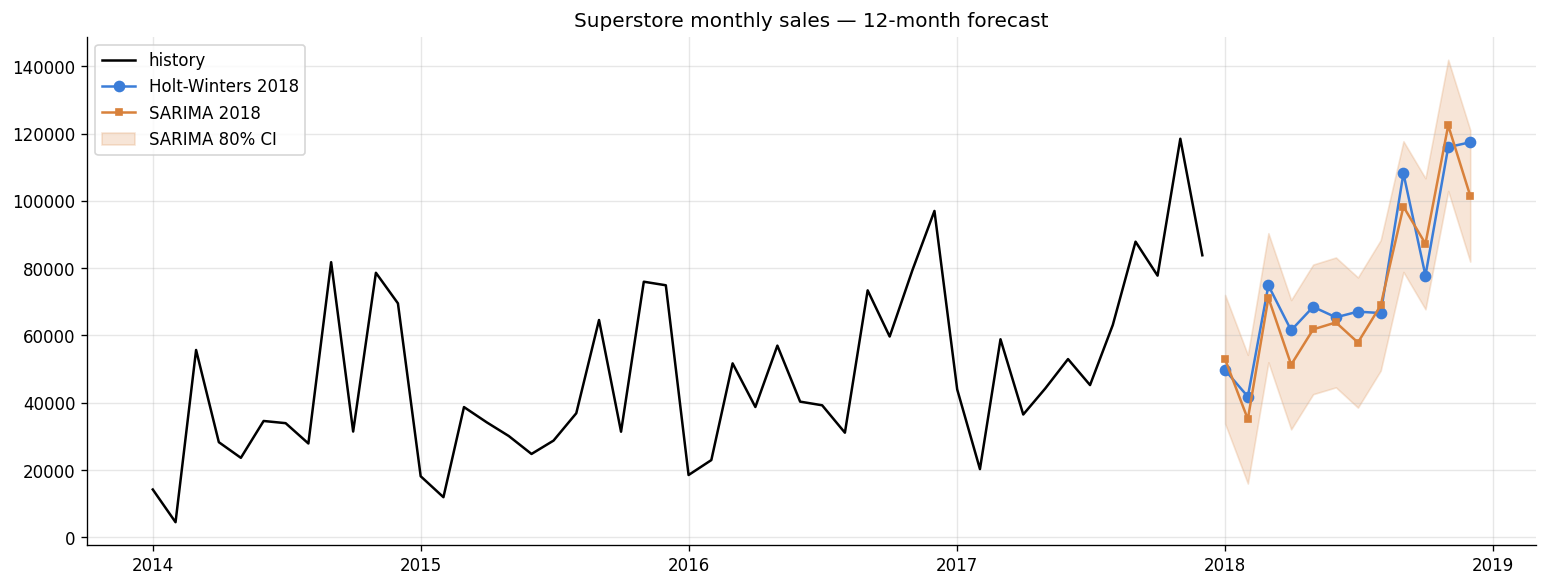
\includegraphics[width=0.95\linewidth]{04_final_forecast.png}
  \caption{History plus the 12-month-ahead forecast: Holt--Winters point
  forecast and the SARIMA 80\% interval.}
  \label{fig:fc-final}
\end{figure}
The next 12 months are projected at \textbf{\$914{,}903}, against
\$733{,}215 realised in the last full year (2017) — a projected
\textbf{+24.8\%} year-on-year. Table~\ref{tab:cat-forecast} breaks this
down by product category (each fit with its own Holt--Winters model on
that category's monthly series).
\begin{table}[H]
  \centering
  \caption{Per-category 2018 projection (Holt--Winters).}
  \label{tab:cat-forecast}
  \begin{tabular}{@{}lrrr@{}}
    \toprule
    Category & 2017 actual (\$) & 2018 projected (\$) & Growth \\
    \midrule
    Office Supplies & 246{,}097 & 326{,}734 & \textbf{+32.8\%} \\
    Furniture       & 215{,}387 & 245{,}463 & +14.0\% \\
    Technology      & 271{,}731 & 272{,}220 & +0.2\% \\
    \bottomrule
  \end{tabular}
\end{table}

\subsection{Residual diagnostics}
\begin{figure}[H]
  \centering
  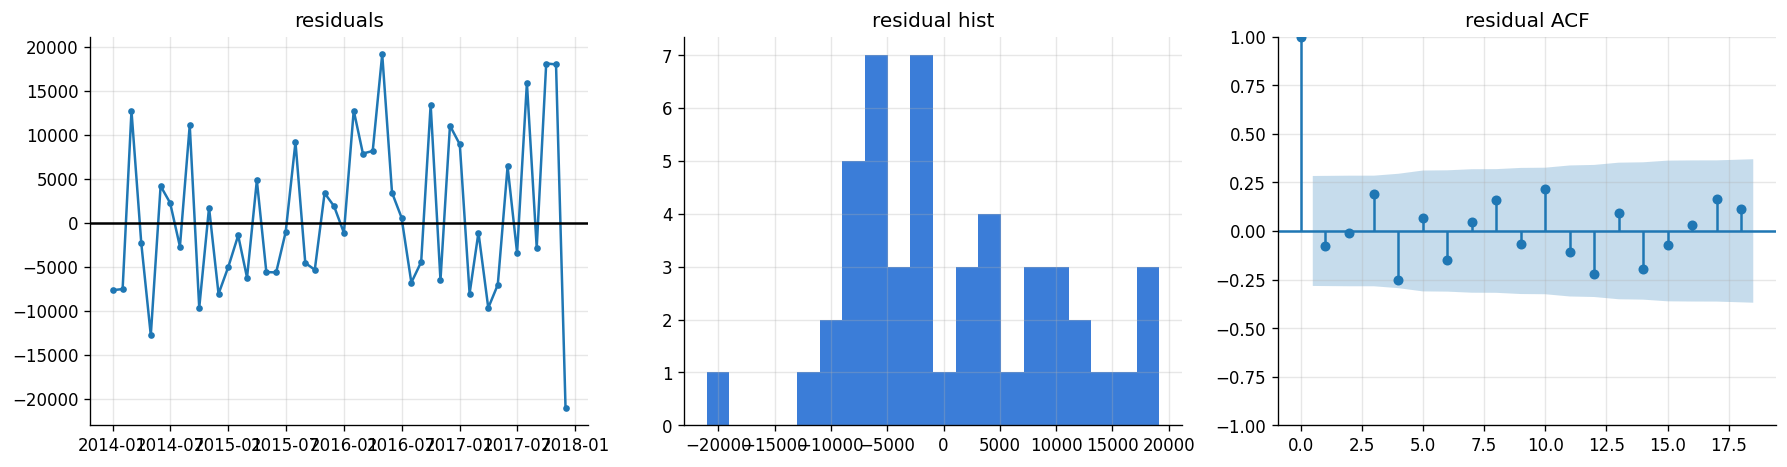
\includegraphics[width=0.95\linewidth]{04_residual_diagnostics.png}
  \caption{Holt--Winters in-sample residuals: time plot, histogram, and
  ACF.}
  \label{fig:fc-resid}
\end{figure}
The Ljung--Box statistic (\cref{eq:ljungbox}) at lag 12 is $Q_{LB}=16.11$,
$p=0.186$ — we fail to reject the null of no residual autocorrelation,
i.e.\ the fitted Holt--Winters model has not left obviously exploitable
structure in its residuals, a reasonable (if not definitive, given
$T=48$) check of adequacy.

\section{Interpretation}
Three points carry forward. First, the ADF results
(\cref{tab:adf}) justify the modelling choice made throughout this
chapter: the series' seasonal \emph{shape}, not only its trend, needs
explicit estimation, which is exactly what both Holt--Winters'
seasonal state $s_t$ and SARIMA's $(P,D,Q)_{12}$ terms provide, and is
why a naive linear-trend-only model is not attempted. Second, the
disagreement between the single hold-out split and the 8-fold rolling
backtest on which of Holt--Winters/SARIMA is "better" is not noise to be
explained away — it is the expected behaviour of a short series with
few independent forecast origins, and is the reason this report reports
\emph{both} evaluations rather than picking whichever looks best. Third,
the practical takeaway for the business is directional, not a claim of
precision: total sales are projected up by roughly a quarter next year,
but growth is sharply uneven by category — Office Supplies is
accelerating, Technology is flat — which is a materially different and
more actionable statement than a single store-wide growth number, and
motivates category-aware inventory/staffing planning rather than a
uniform +25\% assumption.

\chapter{Supervised Models: Profit and Loss at the Line Level}
\label{ch:models}

\section{Theory}

\subsection{Regularised linear regression}
Ordinary least squares fits $\hat y = \mathbf{x}^\top\boldsymbol\beta$ by
minimising the residual sum of squares
$\sum_i (y_i - \mathbf{x}_i^\top\boldsymbol\beta)^2$. With $p=32$
features, several of them one-hot-expanded and correlated (e.g.\
\texttt{Discount} and \texttt{discount\_bucket}), OLS coefficients can
have high variance. \textbf{Ridge regression} adds an $L_2$ penalty,
\begin{equation}
  \hat{\boldsymbol\beta}_{\text{ridge}} = \arg\min_{\boldsymbol\beta}
  \left\{ \sum_{i=1}^n (y_i - \mathbf{x}_i^\top\boldsymbol\beta)^2
          + \lambda \lVert\boldsymbol\beta\rVert_2^2 \right\},
  \label{eq:ridge}
\end{equation}
which shrinks coefficients toward zero and has closed form
$\hat{\boldsymbol\beta}_{\text{ridge}} = (\mathbf{X}^\top\mathbf{X} +
\lambda I)^{-1}\mathbf{X}^\top\mathbf{y}$ — the $\lambda I$ term also
fixes the numerical instability OLS has when $\mathbf{X}^\top\mathbf{X}$
is near-singular, exactly the situation created by correlated dummy
columns. Ridge is used here as the interpretable linear baseline against
which the non-linear ensembles are compared.

\subsection{Bagging and random forests}
\textbf{Bootstrap aggregation (bagging)} reduces the variance of an
unstable base learner (a deep decision tree) by averaging it over $B$
bootstrap resamples of the training data: $\hat f_{\text{bag}}(\mathbf x)
= \frac1B\sum_{b=1}^B \hat f_b(\mathbf x)$. If the $B$ trees had
i.i.d.\ errors, averaging would reduce variance by a factor of $B$; in
practice, trees trained on bootstrap-resampled copies of the \emph{same}
data are positively correlated with pairwise correlation $\rho$, giving
\begin{equation}
  \mathrm{Var}\bigl(\hat f_{\text{bag}}(\mathbf x)\bigr)
    = \rho\,\sigma^2 + \frac{1-\rho}{B}\sigma^2,
  \label{eq:bagging-variance}
\end{equation}
where $\sigma^2$ is a single tree's variance. As $B\to\infty$ the second
term vanishes but the first, $\rho\sigma^2$, remains — so reducing
inter-tree correlation $\rho$ is what actually matters once $B$ is large
enough. \textbf{Random forests} reduce $\rho$ directly: at every split,
only a random subset of $\sqrt p$ (classification) or $p/3$ (regression)
candidate features is considered, forcing different trees to use
different features and decorrelating them beyond what bootstrap resampling
alone achieves. This is why random forests are a strong, low-effort
baseline on tabular data with mixed numeric/categorical features and
non-linear, interaction-heavy structure such as the discount-profit
relationship of \cref{ch:eda}.

\subsection{Gradient boosting}
Where bagging averages independently-grown trees, \textbf{gradient
boosting} grows trees \emph{sequentially}, each one correcting the
current ensemble's errors. Given a differentiable loss
$L(y,F(\mathbf x))$ (squared error for regression here), boosting is
stagewise functional gradient descent: at stage $m$, compute the
pseudo-residuals
\begin{equation}
  r_{im} = -\left.\frac{\partial L(y_i, F(\mathbf x_i))}{\partial F(\mathbf x_i)}\right|_{F=F_{m-1}}
  \label{eq:boost-residual}
\end{equation}
(for squared error, $r_{im}=y_i - F_{m-1}(\mathbf x_i)$, the ordinary
residual), fit a shallow regression tree $h_m$ to predict $r_{im}$ from
$\mathbf x_i$, and update
\begin{equation}
  F_m(\mathbf x) = F_{m-1}(\mathbf x) + \nu\, h_m(\mathbf x),
  \label{eq:boost-update}
\end{equation}
with a small learning rate $\nu<1$ (\emph{shrinkage}) that trades more
boosting stages for better generalisation by taking smaller steps. Unlike
random forests, gradient boosting can in principle drive training error
arbitrarily low and therefore overfits more readily; its typical
signature relative to bagging is lower bias but higher variance without
careful tuning, which is consistent with the regression results below
(GradBoost achieves the best $R^2$ but not the best MAE).

\subsection{Logistic regression and class imbalance}
For the binary target $y\in\{0,1\}$ (\texttt{is\_loss}), logistic
regression models $\Pr(y=1\mid\mathbf x) = \sigma(\mathbf
x^\top\boldsymbol\beta)$ with the logistic sigmoid
$\sigma(z)=1/(1+e^{-z})$, fit by maximising the Bernoulli log-likelihood,
equivalently minimising the log-loss
\begin{equation}
  \mathcal L(\boldsymbol\beta) = -\sum_{i=1}^n
    \bigl[y_i \log \hat p_i + (1-y_i)\log(1-\hat p_i)\bigr],
  \qquad \hat p_i = \sigma(\mathbf x_i^\top\boldsymbol\beta).
  \label{eq:logloss}
\end{equation}
The classification target here is imbalanced (18.7\% positive), so an
unweighted classifier can minimise \cref{eq:logloss} by being mediocre
on the minority (loss-making) class while still achieving low average
loss. \emph{Class weighting} reweights each term of
\cref{eq:logloss} by $w_{y_i} = n / (K\, n_{y_i})$ (inverse class
frequency, $K=2$ classes), so a mistake on a rare loss-making line costs
as much in expectation as a mistake on a common profitable one; all three
non-dummy classifiers in this chapter use \texttt{class\_weight="balanced"}.

\subsection{Classification evaluation under imbalance}
For a threshold $t$ on predicted probability $\hat p$, predictions
$\hat y = \mathbb 1[\hat p \geq t]$ induce a confusion matrix with true
positives $TP$, false positives $FP$, false negatives $FN$, true
negatives $TN$, from which
\begin{equation}
  \mathrm{Precision} = \frac{TP}{TP+FP}, \quad
  \mathrm{Recall} = \frac{TP}{TP+FN}, \quad
  F_1 = \frac{2\cdot\mathrm{Precision}\cdot\mathrm{Recall}}{\mathrm{Precision}+\mathrm{Recall}}.
  \label{eq:prf1}
\end{equation}
The \textbf{ROC curve} plots recall (true-positive rate) against the
false-positive rate $FP/(FP+TN)$ as $t$ varies; the area under it, ROC-AUC,
has the clean probabilistic interpretation
$\mathrm{AUC} = \Pr(\hat p_{+} > \hat p_{-})$ for a randomly drawn
positive and negative example — the probability the model ranks a random
loss-making line above a random profitable one. Under strong class
imbalance, ROC-AUC can look deceptively high because the false-positive
\emph{rate} denominator is dominated by the large negative class; the
\textbf{precision-recall curve} and its area (\textbf{PR-AUC}) are more
informative here because precision directly reflects how many of the
model's loss-flags are real losses, which is what a business decision
(e.g.\ "should we renegotiate this order") actually needs. \textbf{Model
calibration} additionally asks whether $\hat p$ is a trustworthy
probability, not just a good ranking score: a perfectly calibrated model
has $\Pr(y=1 \mid \hat p = q) = q$ for every $q$, visualised by binning
predictions and plotting observed frequency against mean predicted
probability per bin.

\subsection{Permutation feature importance}
For a fitted model $\hat f$ and a chosen scoring function $S$ (e.g.\
negative MAE, or average precision), the permutation importance of
feature $j$ is
\begin{equation}
  \mathrm{PI}_j = S\bigl(\mathbf y, \hat f(\mathbf X)\bigr)
                - \frac1R\sum_{r=1}^R S\bigl(\mathbf y, \hat f(\mathbf X^{(j,r)})\bigr),
  \label{eq:permimp}
\end{equation}
where $\mathbf X^{(j,r)}$ is $\mathbf X$ with column $j$ independently
shuffled (breaking its relationship with $\mathbf y$ while preserving its
marginal distribution) on repeat $r$, averaged over $R$ repeats to reduce
noise. Unlike a tree ensemble's built-in impurity-based importance, this
is model-agnostic, computed on held-out data (so it reflects
generalisation, not just training fit), and directly interpretable in the
scoring metric's own units. Its main caveat is that importance is
\emph{split} between strongly correlated features (permuting one of two
near-duplicate columns barely hurts the score because the model can
still use the other), which is directly relevant here since
\texttt{Discount} and \texttt{discount\_bucket} are derived from the same
underlying quantity.

\section{Method}
Both tasks use the 32-column matrix $\mathbf X$ of \cref{ch:features}
(categoricals one-hot encoded with rare-level collapsing inside an
\texttt{sklearn} \texttt{Pipeline}; numerics standardised only for the
scale-sensitive linear models). The split is \textbf{temporal, not
random}: train on order lines with \texttt{Order Date} $<$ 2017-01-01
(6,682 rows), test on 2017 (3,312 rows) — the model is evaluated on a
genuinely future year it never saw, consistent with how it would be
deployed. Four regressors (dummy-mean, Ridge, RandomForest,
GradientBoosting) target \texttt{Profit}; four classifiers (dummy-prior,
class-weighted LogisticRegression, RandomForest, GradientBoosting) target
\texttt{is\_loss}. The classification decision threshold is additionally
tuned on the test set by grid search over $[0.05,0.95]$ to maximise $F_1$
(\cref{eq:prf1}) — a simplification made explicit here: in a real
deployment this threshold should be chosen on a separate validation slice,
not the final test set, to avoid a (mild) form of the same leakage risk
discussed in \cref{ch:features}.

\section{Results}

\subsection{Profit regression}
\begin{table}[H]
  \centering
  \caption{Profit regression, 2017 hold-out.}
  \label{tab:reg-results}
  \begin{tabular}{@{}lrrr@{}}
    \toprule
    Model & MAE (\$) & RMSE (\$) & $R^2$ \\
    \midrule
    \textbf{RandomForest} & \textbf{21.42} & 139.24 & 0.668 \\
    GradBoost              & 25.54 & \textbf{113.42} & \textbf{0.780} \\
    Ridge                  & 58.66 & 183.11 & 0.427 \\
    Dummy (mean)           & 64.68 & 241.83 & $\approx$0 \\
    \bottomrule
  \end{tabular}
\end{table}
RandomForest has the lowest MAE, GradBoost the best RMSE/$R^2$ — per the
bagging-vs-boosting theory above, GradBoost fits the bulk of the
distribution tighter (lower RMSE, which penalises the largest errors most)
while RandomForest is more robust on typical-sized errors (lower MAE);
both crush the linear Ridge baseline, confirming the profit-generating
process is substantially non-linear (consistent with the discount
\emph{threshold} effect of \cref{ch:eda}, which no linear term can
represent well).
\begin{figure}[H]
  \centering
  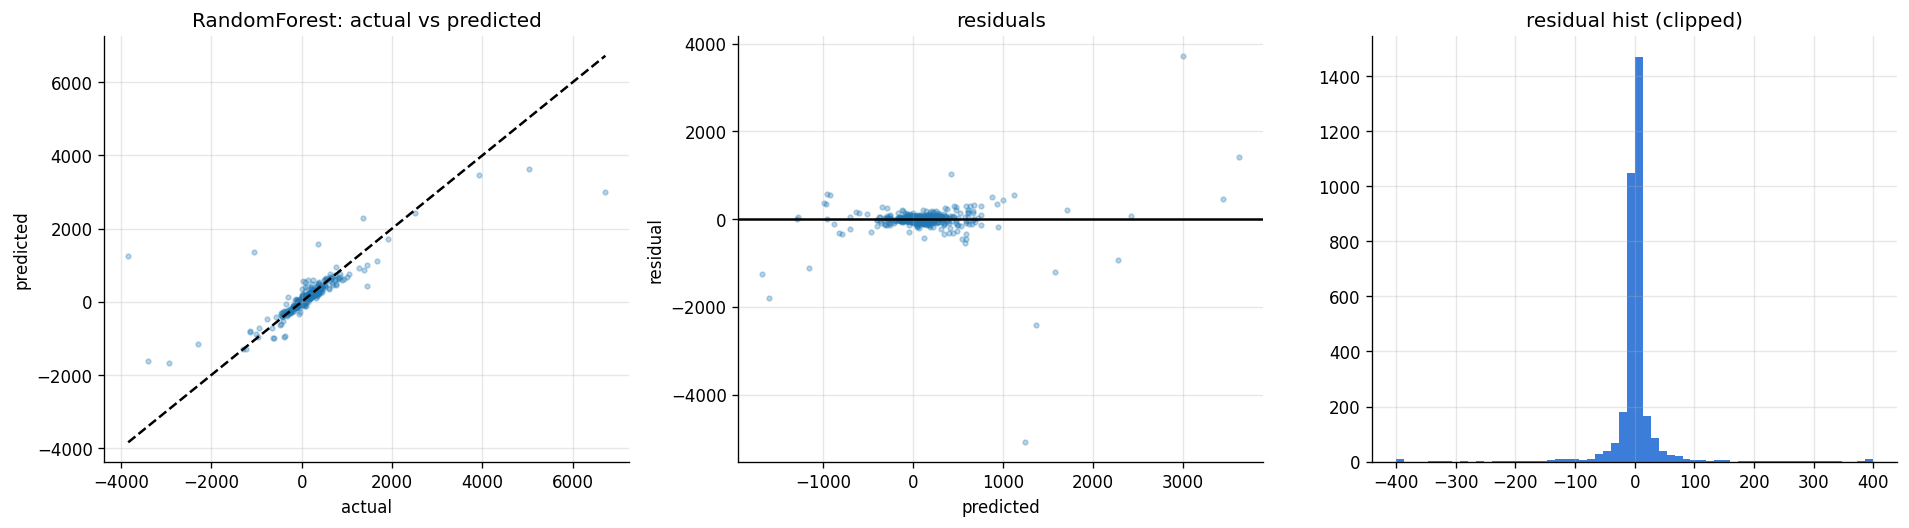
\includegraphics[width=0.95\linewidth]{05_regression_diagnostics.png}
  \caption{RandomForest regression diagnostics: predicted vs.\ actual,
  residuals vs.\ predicted, and the residual distribution.}
  \label{fig:reg-diag}
\end{figure}
\begin{figure}[H]
  \centering
  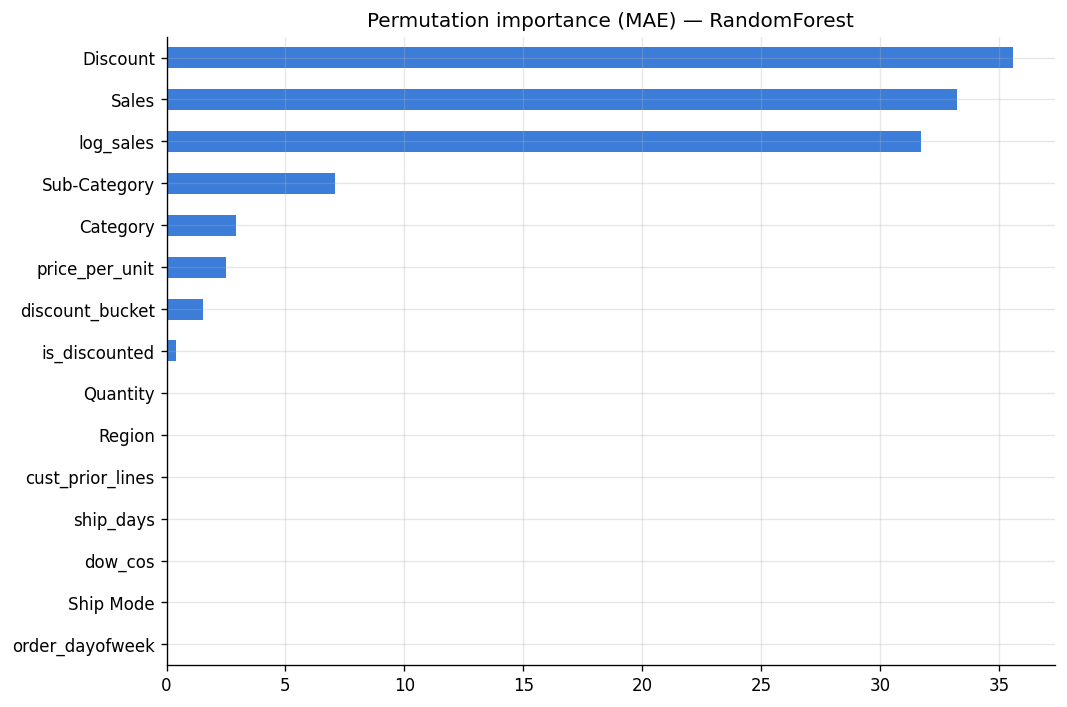
\includegraphics[width=0.75\linewidth]{05_regression_importance.png}
  \caption{Permutation importance (\cref{eq:permimp}, scoring = negative
  MAE) for the RandomForest regressor.}
  \label{fig:reg-imp}
\end{figure}
\texttt{Discount} (35.6), \texttt{Sales} (33.2) and \texttt{log\_sales}
(31.7) dominate; \texttt{Sub-Category} (7.1) is a distant fourth. Error
concentrates in the highest-ticket sub-categories — Copiers (\$367 mean
absolute error) and Machines (\$356) — where a single order's discount
swings profit by hundreds of dollars, versus \$21--\$79 for every other
sub-category shown.

\subsection{Loss classification}
\begin{table}[H]
  \centering
  \caption{Loss-line classification, 2017 hold-out.}
  \label{tab:clf-results}
  \begin{tabular}{@{}lrrr@{}}
    \toprule
    Model & ROC-AUC & PR-AUC & $F_1$ (t=0.5) \\
    \midrule
    \textbf{RandomForest} & 0.988 & \textbf{0.956} & \textbf{0.865} \\
    GradBoost              & 0.986 & 0.947 & 0.804 \\
    LogReg (balanced)      & 0.985 & 0.945 & 0.828 \\
    Dummy (prior)          & 0.500 & 0.187 & 0.000 \\
    \bottomrule
  \end{tabular}
\end{table}
All three fitted models are far above the 0.187 PR-AUC a model that
ignores the features entirely would achieve by always predicting the
base rate (Dummy's PR-AUC exactly equals the positive-class prevalence,
as \cref{eq:permimp}'s baseline case would predict). RandomForest is
best on every metric. At its best-$F_1$ threshold ($t=0.50$, $F_1=0.865$)
its classification report is:
\begin{center}
\begin{tabular}{lrrrr}
\toprule
 & Precision & Recall & $F_1$ & Support \\
\midrule
profit & 0.96 & 0.98 & 0.97 & 2{,}692 \\
loss   & 0.91 & 0.83 & 0.86 & 620 \\
\bottomrule
\end{tabular}
\end{center}
\begin{figure}[H]
  \centering
  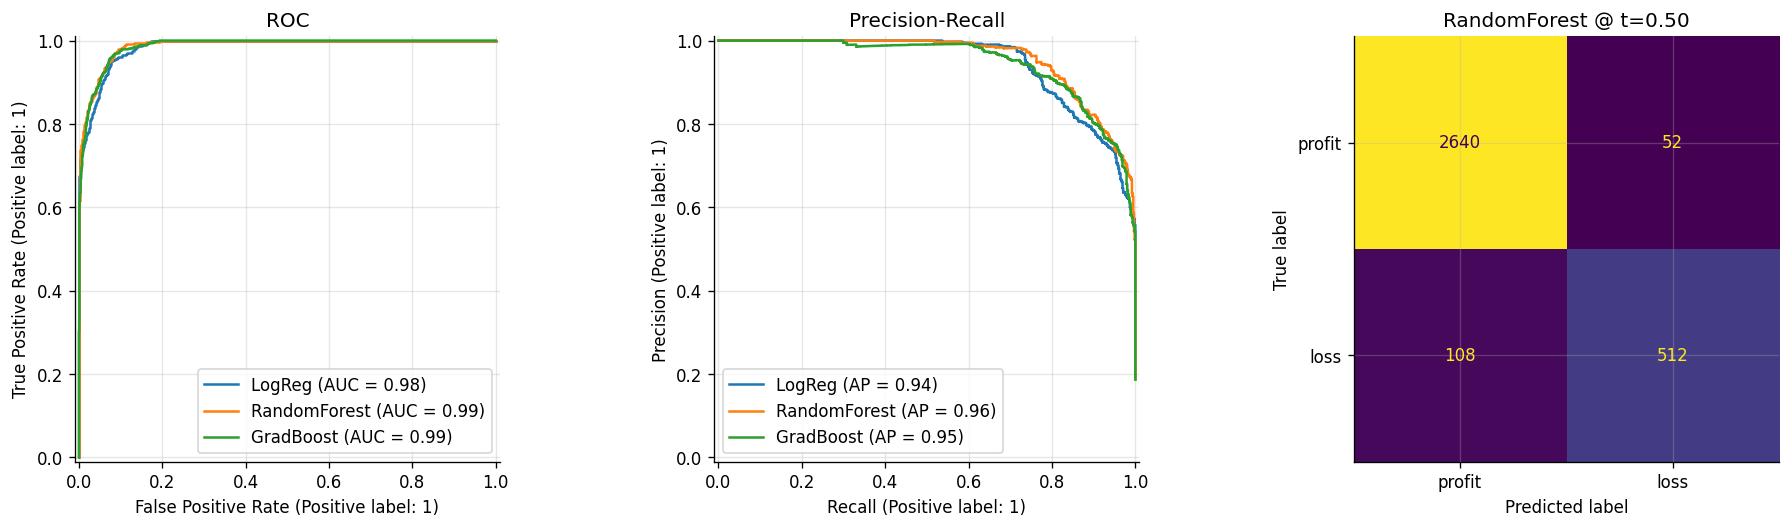
\includegraphics[width=0.95\linewidth]{05_classification_curves.png}
  \caption{ROC (left), precision-recall (middle) and confusion matrix
  (right, RandomForest at $t{=}0.50$).}
  \label{fig:clf-curves}
\end{figure}
\begin{figure}[H]
  \centering
  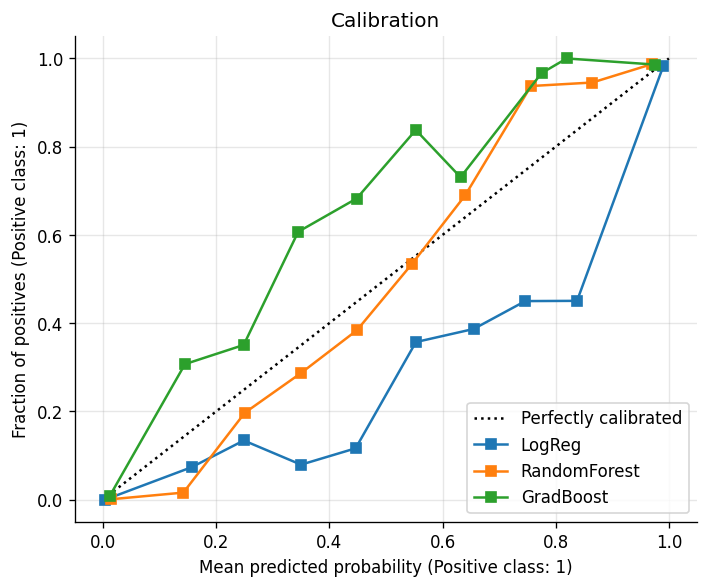
\includegraphics[width=0.55\linewidth]{05_calibration.png}
  \caption{Calibration curves: observed vs.\ predicted positive rate by
  probability decile.}
  \label{fig:clf-calib}
\end{figure}
\begin{figure}[H]
  \centering
  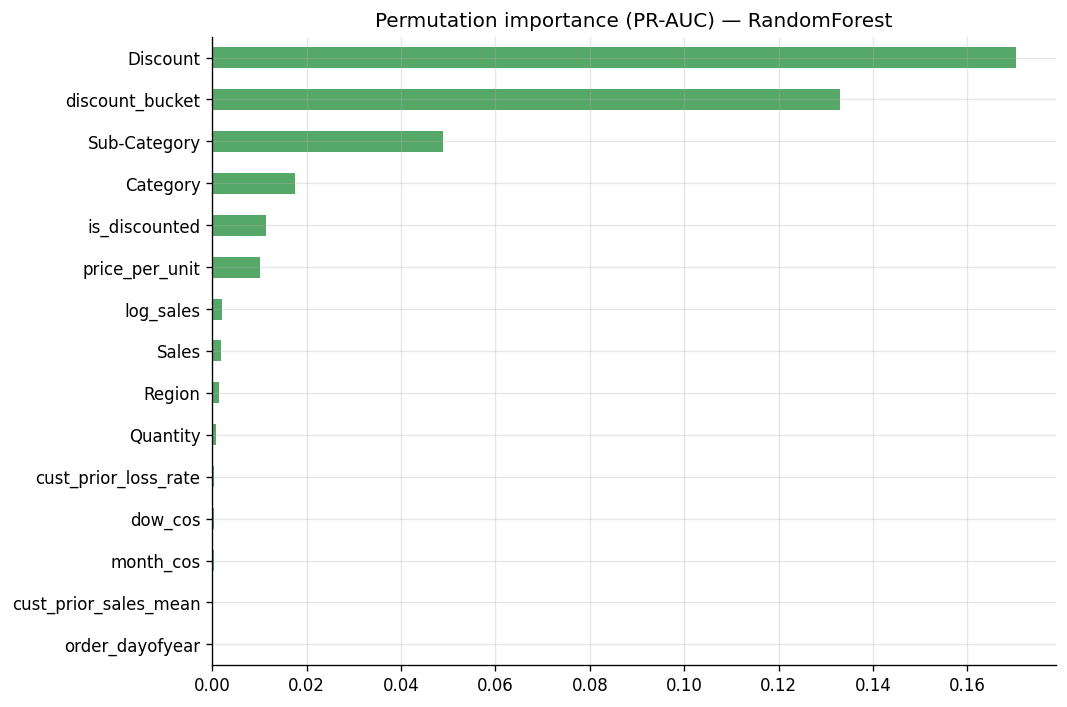
\includegraphics[width=0.75\linewidth]{05_classification_importance.png}
  \caption{Permutation importance (scoring = average precision) for the
  RandomForest classifier.}
  \label{fig:clf-imp}
\end{figure}
\texttt{Discount} (0.170) and \texttt{discount\_bucket} (0.133) again
dominate, jointly far ahead of \texttt{Sub-Category} (0.049) — the same
two-feature dominance seen in the regression task, as expected since both
targets are driven by the same underlying discount-threshold mechanism.

\subsection{Business framing}
Translating the classifier into dollar terms on the 2017 test set:
realised profit was \$93{,}439; of the total loss on loss-making lines,
flagged lines captured \$50{,}138 (a \textbf{93.1\% catch rate} by
dollar value) against \$3{,}699 missed, at the cost of putting
\$1{,}358 of genuinely profitable business "at risk" from unnecessary
renegotiation (false positives) — a roughly 37:1 ratio of dollars
correctly caught to dollars put at risk.

\section{Interpretation}
The regression and classification results triangulate on the same
mechanism identified qualitatively in \cref{ch:eda} and made numeric in
\cref{ch:features}: \textbf{discount depth is, by a wide margin, the
dominant driver of both how much profit a line makes and whether it
loses money at all}. This is reassuring from a model-validity standpoint
— two independently trained model families (an ensemble regressor and an
ensemble classifier, on different targets) converge on the same top
features — and, more importantly, it is actionable: a discount-governance
rule (e.g.\ a required approval step for discounts above roughly 30\%,
per \cref{tab:discount-bucket}) would target the overwhelming majority of
the loss identified by the model, and the classifier itself offers a
concrete, auditable early-warning signal (93\% dollar-recall on a future
year) for flagging specific at-risk order lines before or as they are
placed, rather than only after the fact in a quarterly profit review.


\end{document}
